\section{Single phase consolidation}
Let us begin by introducing a few governing equations.

\subsubsection*{Fluid mass and momentum balance}
Linear momentum balance for the fluid follows Darcy:

\begin{equation}
{v}_{ri}=\phi \left( {{v}_{i}}-{{v}_{si}} \right)=-\frac{{{k}_{ij}}}{\mu }\left( \frac{\partial p}{\partial {{x}_{j}}}+\rho {{g}_{j}} \right),
\label{eqch14:genmass}
\end{equation}

for the intrinsic permeability, ${{k}_{ij}}$, dynamic viscosity, $\mu $, and density, $\rho $. The subscript $r$ considers that fluid velocity is relative to motion of the deformable solid (${{v}_{si}}$), so that ${{v}_{i}}$ is absolute fluid velocity, and ${{v}_{ri}}$ is relative. Conservation of fluid mass requires,

\begin{equation}
\frac{\partial }{\partial t}\left( \phi \rho  \right)+\frac{\partial }{\partial {{x}_{i}}}\left( \phi \rho {{v}_{i}} \right)=0.
\end{equation}
	
Fluid properties are functions of temperature and pressure. The fluid density time derivative appearing in the mass balance equation may be expanded to

\begin{equation}
\frac{d\rho}{dt}=\rho \left( \frac{1}{K_{f}^{p}}\frac{dp}{dt}-\frac{1}{K_{f}^{T}}\frac{dT}{dt} \right),
\end{equation}
	
with fluid compressibility given by $1/K_{f}^{p}={{\left. \left( 1/\rho  \right)\left( \partial \rho /\partial p \right) \right|}_{T}}$ and for the fluid thermal expansion coefficient $1/K_{f}^{T}=-{{\left. \left( 1/\rho  \right)\left( \partial \rho /\partial T \right) \right|}_{p}}$. In these definitions we utilize moduli ($K$ = inverse compressibility). Also, because thermal effects are not considered in these examples, the temperature dependence may be neglected. Utilizing the Lagrangian total derivative of a component relative to the moving solid, ${{d}_{s}}/dt=\partial /\partial t+{{v}_{si}}\partial /\partial {{x}_{i}}$, and a moving fluid, ${{d}_{f}}/dt=\partial /\partial t+{{v}_{fi}}\partial /\partial {{x}_{i}}$, substituting for absolute fluid velocity and dividing through by density gives,

\begin{equation}
\phi \left( \frac{1}{K_{f}^{p}}\frac{dp}{dt}+\frac{{{d}_{s}}\phi }{dt}+\frac{\partial {{v}_{si}}}{\partial {{x}_{i}}} \right)=-\frac{\partial }{\partial {{x}_{i}}}\left( {{v}_{ri}} \right).
\end{equation}
	
To obtain the porosity time derivative, we expand the solid mass balance to obtain

\begin{equation}
\frac{{{d}_{s}}\phi }{dt}=\frac{\left( 1-\phi  \right)}{{{\rho }_{s}}}\frac{\partial {{\rho }_{s}}}{\partial t}+\left( 1-\phi  \right)\frac{\partial {{v}_{si}}}{\partial {{x}_{i}}}.
\end{equation}
	
Substituting this gives,

\begin{equation}
\frac{\phi }{K_{f}^{p}}\frac{dp}{dt}+\left[ \frac{\partial {{v}_{si}}}{\partial {{x}_{i}}}+\frac{\left( 1-{{\rho }_{s}} \right)}{{{\rho }_{s}}}\frac{\partial {{\rho }_{s}}}{\partial t} \right]=-\frac{\partial }{\partial {{x}_{i}}}\left( {{v}_{ri}} \right).
\end{equation}
	
Utilizing Biot's formulation to represent the solid density time derivative and assuming small strain yields the full fluid mass balance (\cite{KhaliliSelvadurai:03} and \cite{RutEtAl:01}),

\begin{equation}
\left( \frac{\phi }{K_{f}^{p}}+\overbrace{\frac{\left( \alpha -\phi  \right)}{{{K}_{g}}}}^{A} \right)\frac{dp}{dt}+\overbrace{\alpha \frac{\partial {{v}_{si}}}{\partial {{x}_{i}}}}^{B}=-\frac{\partial }{\partial {{x}_{i}}}\left( {{v}_{ri}} \right),
\label{eqch14:flmass}
\end{equation}
	
where ${{K}_{g}}$ is the solid grain bulk modulus, and $\alpha$ is the Biot-Willis coefficient ($\alpha =1-K/{{K}_{g}}$ in an ideal, fully interconnected porous media). The bracketed terms $A$ and $B$ represent important couplings from the mechanical system to that of the fluid. All are vital in the HM procedure and without them the equation simplifies to a standard fluid flow equation with fluid compressibility storage in the pressure time derivative. 

\subsubsection*{Solid momentum balance}

We begin with the concept of effective stress,

\begin{equation}
\sigma {{'}_{ij}}={{\sigma }_{ij}}+\alpha p{{\delta }_{ij}},
\end{equation}

for the effective stress, $\sigma '$, and the total stress, $\sigma$; negative in compression. Balance of linear momentum is defined by,

\begin{equation}
\frac{\partial {{\sigma }_{ij}}}{\partial {{x}_{j}}}+{{F}_{i}}=0,
\end{equation}

for the body force, $F=\rho _m \text{g}$ and where $\rho _m =\phi \rho _f + (1-\phi )\rho _s$ is density of the mixture. From the definition of strain, ${{\varepsilon }_{ij}}=\left( \partial {{u}_{i}}/\partial {{x}_{j}}+\partial {{u}_{j}}/\partial {{x}_{i}} \right)/2$, and an arbitrary stress-strain relationship of the form $\mathbf{\sigma }=\mathbf{D\varepsilon }\left( \mathbf{u} \right)$, we write the displacement formulation of mechanical equilibrium (neglecting thermal effects) for isotropic linear elasticity,

\begin{equation}
\frac{\partial }{\partial {{x}_{j}}}\left[ G\frac{\partial {{u}_{i}}}{\partial {{x}_{j}}}+\left( \lambda +G \right)\frac{\partial {{u}_{j}}}{\partial {{x}_{i}}}-\alpha p{{\delta }_{ij}} \right]+{{F}_{i}}=0,
\label{eqch14:mequil}
\end{equation}

where $G$ and $\lambda$ are the Lam� constants. Changes to the fluid system are therefore visited in mechanical equilibrium via the effective stress.

\subsubsection*{Numerical solution scheme}
The numerical solution of Eqs. \ref{eqch14:flmass} and \ref{eqch14:mequil} can be obtained with any convenient method. In these benchmarks, we use a standard Galerkin finite element spatial discretization with time discretization following a generalized first order finite difference scheme, as implemented in OpenGeoSys. Note that Eq. \ref{eqch14:mequil} is an equilibrium equation, and has no time dependency other than that imposed by coupling terms to fluid behavior. The result is a set of coupled linear equations in pressure, $p$, and solid displacement, $u$. The two equations may be solved sequentially and iteratively, or monolithically as a single system. We present results using both solution schemes in the following benchmarks.

%-------------------------------------------------------------------------
%-------------------------------------------------------------------------

\subsection{Background}
\subsubsection*{Mass balance equation}
Consider two-phase flow in porous media, e.g liquid (denoted by $l$) and gas (denoted by $g$). For each phase in two-phase fluid flow, mass conservation is given by the following equation:

\begin{align}
\pD{}{t}\left(\poro S^g\dens_k^g+\poro S^l\dens_k^l\right)+\nabla \cdot \left( \FlxDf_k^g+\FlxDf_k^l\right)=Q_k
\label{eq:massb}
\end{align}

where $S$ is saturation, $\dens$ stands for phase density, $\poro$ is the porosity, $\FlxDf$ is total flux. The subscript $k$ in equation (\ref{eq:massb}) denotes the component, e.g air ($k=a$) or water ($k=w$), within each phase, $\gamma=(g,l)$. For any phase $\gamma=(g,l)$, an advection vector ${{\FlxDf}_A}_k^{\gamma}$ and a diffusion vector  ${{\FlxDf}_D}_k^{\gamma}$ comprise the total flux, i.e

\begin{align}
\FlxDf_k^{\gamma}={{\FlxDf}_A}_k^{\gamma}+{{\FlxDf}_D}_k^{\gamma}
\label{eq:tflx}
\end{align}

According to Darcy's law, the advective part of the total flux may be written as

\begin{align}
{{\FlxDf}_A}_k^{\gamma}=-\dens_k^{\gamma}\dfrac{\perm \RelKa^{\gamma}}{\mu^{\gamma}}\left(\nabla \pres^{\gamma}-\dens^{\gamma} \mathbf g\right)
\label{eq:flx_dc}
\end{align}

where $\perm$ is the intrinsic permeability, $\RelKa^{\gamma}$ is the relative permeability of the phase, and $\mu^{\gamma}$ is the viscosity.

The diffusive part of the total flux is given by Fick's law

\begin{align}
{{\FlxDf}_D}_k^{\gamma}=-\poro \sat^{\gamma}  \dens^{\gamma} {\mathbb D}_k^{\gamma} \nabla \left(\dfrac{\dens_k^{\gamma}}{\dens^{\gamma}}\right)
\label{eq:flx_fk}
\end{align}

where $\mathbb D$ is the diffusion coefficient tensor. Since $\dens^{\gamma} = \dens_a^{\gamma}+\dens_w^{\gamma}$, we have

 \begin{align}
{{\FlxDf}_D}_w^{\gamma}+{{\FlxDf}_D}_a^{\gamma}=\mathbf 0
\label{eq:dufblc}
\end{align}

under the assumption ${\mathbb D}_a^{\gamma}  = {\mathbb D}_w^{\gamma} $.

Consider a water-air mixture. We expand the mass balance equation (\ref{eq:massb}) with the flux defined in equations (\ref{eq:tflx}) based upon the above equations (\ref{eq:tflx}, \ref{eq:flx_dc}, \ref{eq:flx_fk}). For the water component, the diffusive part of the total flux takes the form

\begin{align}
{{\FlxDf}_D}_w^{l}=-\poro \Sat^{l}  \dens^{l} {\mathbb D}_w^{l} \nabla \left(\dfrac{\dens_w^{l}}{\dens^{l}}\right),\quad
{{\FlxDf}_D}_w^{g}=-\poro \Sat^{g}  \dens^{g} {\mathbb D}_w^{g} \nabla \left(\dfrac{\dens_w^{g}}{\dens^{g}}\right)
\label{eq:flx_fkw}
\end{align}

Obviously, ${\mathbb D}_w^{l} = \mathbf 0$. Therefore, the mass balance equation for water component can be written as follows

\begin{align}
\pD{}{t} \left(\poro S^g\dens_w^g+\poro S^l\dens_w^l\right)-
\nabla \cdot \left[\dens_w^{l}\dfrac{\perm \RelKa^{l}}{\mu^{l}}\left(\nabla \pres^{l}-\dens^{l} \mathbf g\right)\right]\nonumber\\
-\nabla \cdot \left[\dens_w^{g}\dfrac{\perm \RelKa^{g}}{\mu^{g}}\left(\nabla \pres^{g}-\dens^{g} \mathbf g\right)\right] -
\nabla \cdot \left[\poro \Sat^{g}  \dens^{g} {\mathbb D}_w^{g} \nabla \left(\dfrac{\dens_w^{g}}{\dens^{g}}\right)\right] = Q_w
\label{eq:massblq}
\end{align}

Since the capillary pressure $\pres^c$  is chosen as one of the two unknowns of equation (\ref{eq:massb}) and $S^g=1-S^l$, equation (\ref{eq:massblq}) becomes

\begin{align}
\poro (\dens_w^l -\dens_w^g)\pD{S^l}{t} +(1 -S^l)\poro \pD{\dens_w^{g}}{t} -
\nabla \cdot \left[\dens_w^{l}\dfrac{\perm \RelKa^{l}}{\mu^{l}}\left(\nabla (\pres^{g}-\pres^{c}) -\dens^{l} \mathbf g\right)\right]\nonumber\\
-\nabla \cdot \left[\dens_w^{g}\dfrac{\perm \RelKa^{g}}{\mu^{g}}\left(\nabla \pres^{g}-\dens^{g} \mathbf g\right)\right] -
\nabla \cdot \left[\poro \Sat^{g}  \dens^{g} {\mathbb D}_w^{g} \nabla \left(\dfrac{\dens_w^{g}}{\dens^{g}}\right)\right] = Q_w
\label{eq:msblq}
\end{align}

Similar to the previous procedure, the diffusion part of the total flux of air component can be written as

\begin{align}
{{\FlxDf}_D}_a^{l}=-\poro \Sat^{l}  \dens^{l} {\mathbb D}_a^{l} \nabla \left(\dfrac{\dens_a^{l}}{\dens^{l}}\right),\quad
{{\FlxDf}_D}_a^{a}=-\poro \Sat^{g}  \dens^{g} {\mathbb D}_a^{g} \nabla \left(\dfrac{\dens_a^{g}}{\dens^{g}}\right)
\label{eq:flx_fka}
\end{align}

The density shift from air component to liquid ${\dens_a^{l}}$ is very small and can be omitted. Therefore, we can assume ${{\FlxDf}_D}_a^{l}\thickapprox0$. As a consequence, the mass balance equation for air component is derived as:

$$\pD{}{t} \left(\poro S^g\dens_a^g\right) -$$
\begin{align}
\nabla \cdot \left[\dens_a^{g}\dfrac{\perm \RelKa^{g}}{\mu^{g}}\left(\nabla \pres^{g}-\dens^{g} \mathbf g\right)\right]-\nabla \cdot \left[\poro \Sat^{g}  \dens^{g} {\mathbb D}_a^{g} \nabla \left(\dfrac{\dens_a^{g}}{\dens^{g}}\right)\right] =Q_a
\label{eq:massba}
\end{align}

Expanding the temporary derivative term of equation (\ref{eq:massba}) yields

$$-\poro \dens_a^g \pD{S^l}{t} + (1 -S^l)\poro \pD{\dens_a^{g}}{t}-$$
\begin{align}
\nabla \cdot \left[\dens_a^{g}\dfrac{\perm \RelKa^{g}}{\mu^{g}}\left(\nabla \pres^{g}-\dens^{g} \mathbf g\right)\right] -
\nabla \cdot \left[\poro \Sat^{g} \dens^{g} {\mathbb D}_a^{g} \nabla \left(\dfrac{\dens_a^{g}}{\dens^{g}}\right)\right] = Q_a
\label{eq:msba}
\end{align}

The mass balance equations (\ref{eq:msblq}) and (\ref{eq:msba}) are exactly the same as described in \cite{SanPesSch:06}.

\subsubsection*{Pressure-pressure (pp) scheme}
Based on the description of isothermal two-phase flow above, (\ref{eq:msblq}) and (\ref{eq:msba}) can be modified in order to obtain governing equation for the isothermal two-phase flow in a porous medium. In this formulation primary variables are gas pressure $\asup{\pres}{g}$, and capilary pressure $\asup{\pres}{c}$.

The basic equations of the isothermal two-phase flow system are:

\begin{align}
\poro \dens_w \pD{S_w}{\pres_c} \dot\pres_c +
\nabla \cdot\left[\dens_w\dfrac{{\perm \RelKa}_{w}}{\mu_w}\left(-\nabla \pres^{g} +
\nabla{\pres}^{c} + \dens_w \mathbf g\right)\right] = Q_w
\end{align}
\begin{align}
- \poro \dens^a \pD{S_w}{\pres_c} \dot\pres_c+
\poro (1 -S_w)\left(\pD{\dens_a}{\pres^g}\dot\pres^g+\pD{\dens_a}{\pres_c}\dot\pres_c\right)+ \nonumber\\
\nabla \cdot \left[\dens_a\dfrac{{\perm \RelKa}_a}{\mu_a} \left(-\nabla\pres^{g} + \dens_a \mathbf g\right) \right] = Q_a
\label{eq:msbl_sim}
\end{align}

\subsubsection*{Pressure-saturation (pS) scheme}
Based on the description of the isothermal two-phase flow above, (\ref{eq:msblq}) and (\ref{eq:msba}) can be modified in order to obtain governing equation for the isothermal two-phase system. Primary variables of this formulation are wetting phase pressure $p_w$, and non-wetting phase saturation $S_{nw}$. The equations are simply algebraic manipulations of those in the previous section.
\subsection{Distributed footing: Poroelastic cube (3D)}
We consider a vertical cross-section through homogeneous soil. Due to symmetry we can limit the investigation to half of the domain. The model domain is then extending 8 meters in length and 5 meters in height. The problem is solved in 2D and 3D space, respectively.

\begin{figure}[!tbh]
\begin{center}
\scalebox{1.0} % Change this value to rescale the drawing.
{
\begin{picture}(380,190)
\put(70,160){\line(1,0){240}}
\put(310,10){\line(0,1){150}}
\multiput(70,10)(0,11){14}{\line(0,1){7}}
\put(75,180){\vector(0,-1){20}}
\put(80,180){\vector(0,-1){20}}
\put(85,180){\vector(0,-1){20}}
\put(90,180){\vector(0,-1){20}}
\put(95,180){\vector(0,-1){20}}
\put(308,165){8}
\put(60,165){0}
\put(55,8){-5}
% BC
% left
\put(5,100){$\frac{\partial p}{\partial x} = 0$}
\put(5,85) {$u_x = 0$}
\put(5,75) {$\sigma_{xy} = 0$}
% top
\put(75,150){$\sigma_{yy}=\sigma_0$}
\put(75,140){$\sigma_{xy}=0$}
\put(180,165){$\sigma_{xy}=\sigma_{yy}=0$}
\put(210,187){\vector(1,0){100}}
\put(175,187){\vector(-1,0){105}}
\put(180,185){$p=0$}
% right
\put(320,100){$\frac{\partial p}{\partial x} = 0$}
\put(320,85) {$u_x = 0$}
\put(320,75) {$\sigma_{xy} = 0$}
% bottom
\put(160,-5){$\frac{\partial p}{\partial y} = 0$ , $u_x=u_y=0$}
\linethickness{2pt}
\put(70,10){\line(1,0){240}}
\end{picture}
}
\end{center}
\caption{Conceptualization of the footing problem. Properties are Young's modulus, $E=3\times 10^{4}$ $N/m^{2}$, Poisson's ratio, $\nu =0.2$, permeability, $k=10^{-10}$ $m^2$, and fluid viscosity, $\mu =10^{-3}$ $Pa\,s$.}
\label{fig-setting}
\end{figure} 

\subsubsection*{Definition}
A strip loading is imposed ($\sigma _{yy}=\sigma _0$ in $x\in [0,1]$), with zero stresses
($\sigma _{yy}=\sigma _{xy}=0$ in $x\in(1,8]$) and zero pressure at the top; no horizontal flux, no horizontal displacements and zero shear stresses at left and right boundaries with no vertical flux and no displacement at the bottom (Fig. \ref{fig-setting}). 

\subsubsection*{Results}
The 3D geometry expands the 2D domain by extruding the 2D shape by 1m in the off-plane direction (\ref{fig_HM3}). Results at the critical step, i.e., the first step, are shown in Fig. \ref{fig:e10}, \ref{fig:e12} and  \ref{fig:e11}. The results produced using the 2D model with triangular elements and the 3D model with tetrahedral elements match each other well, thus providing confidence in higher dimensions.

\begin{figure}[!tbh]
\vspace{-1cm}
\begin{center}
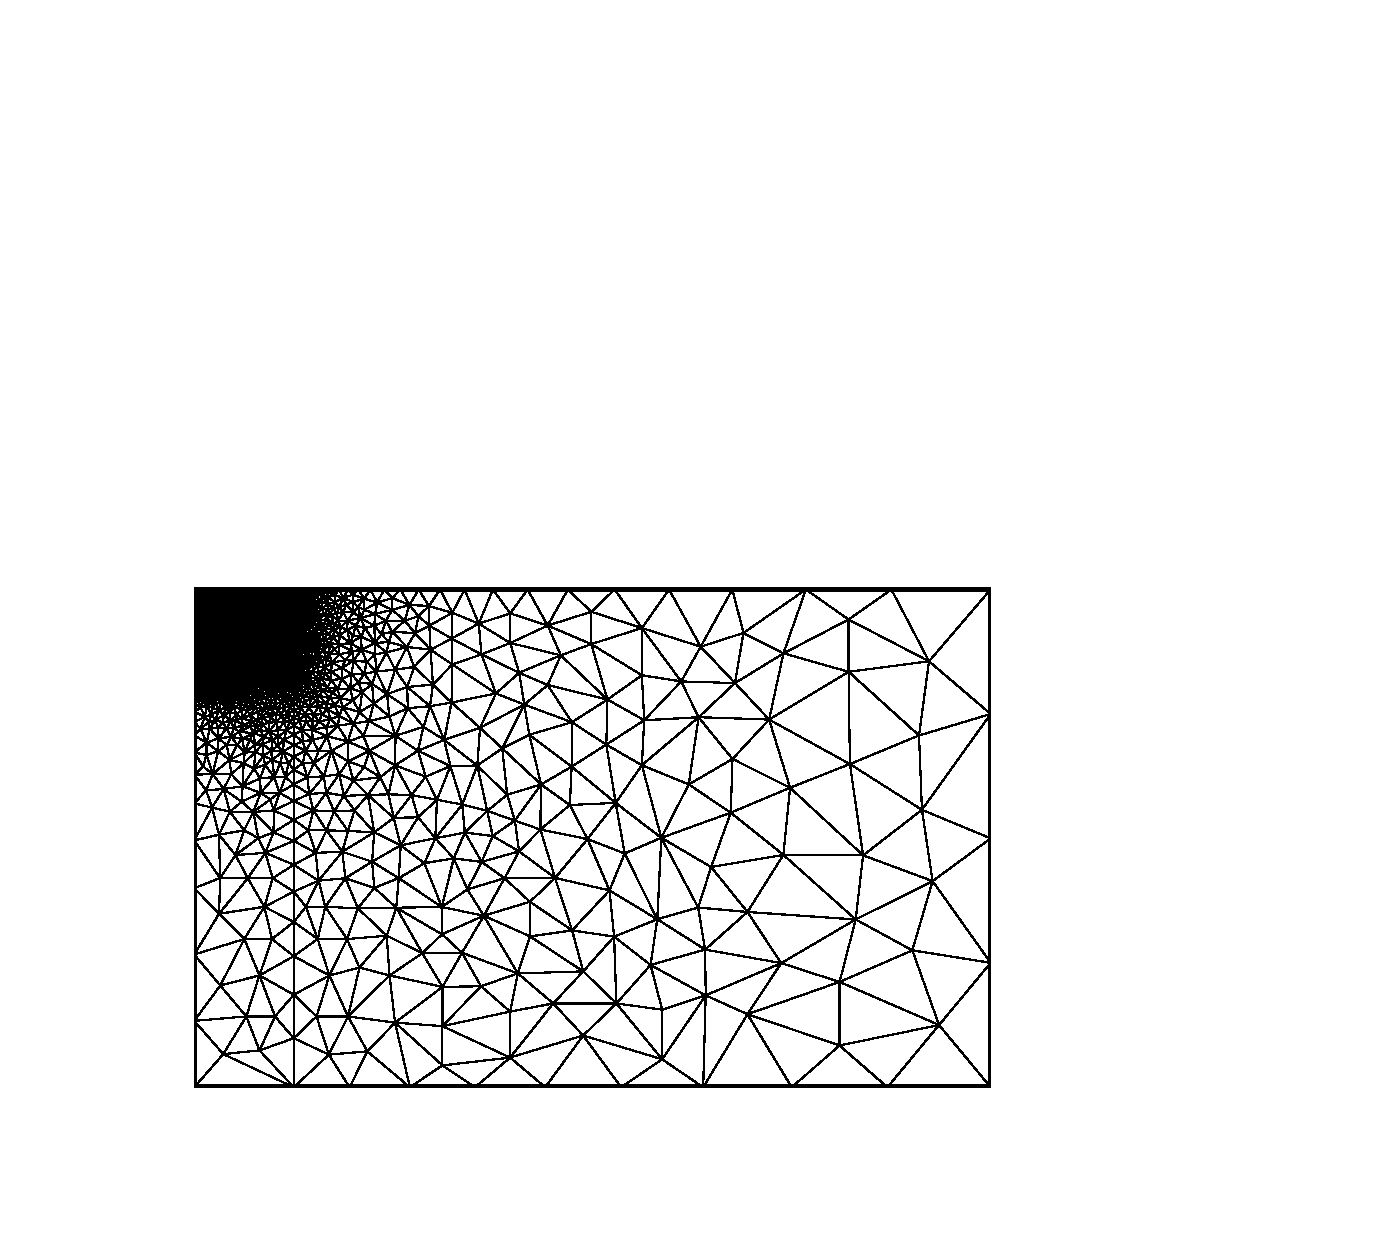
\includegraphics[width=0.54\textwidth]{chapter_14/figures/fig_14_1_4_a}
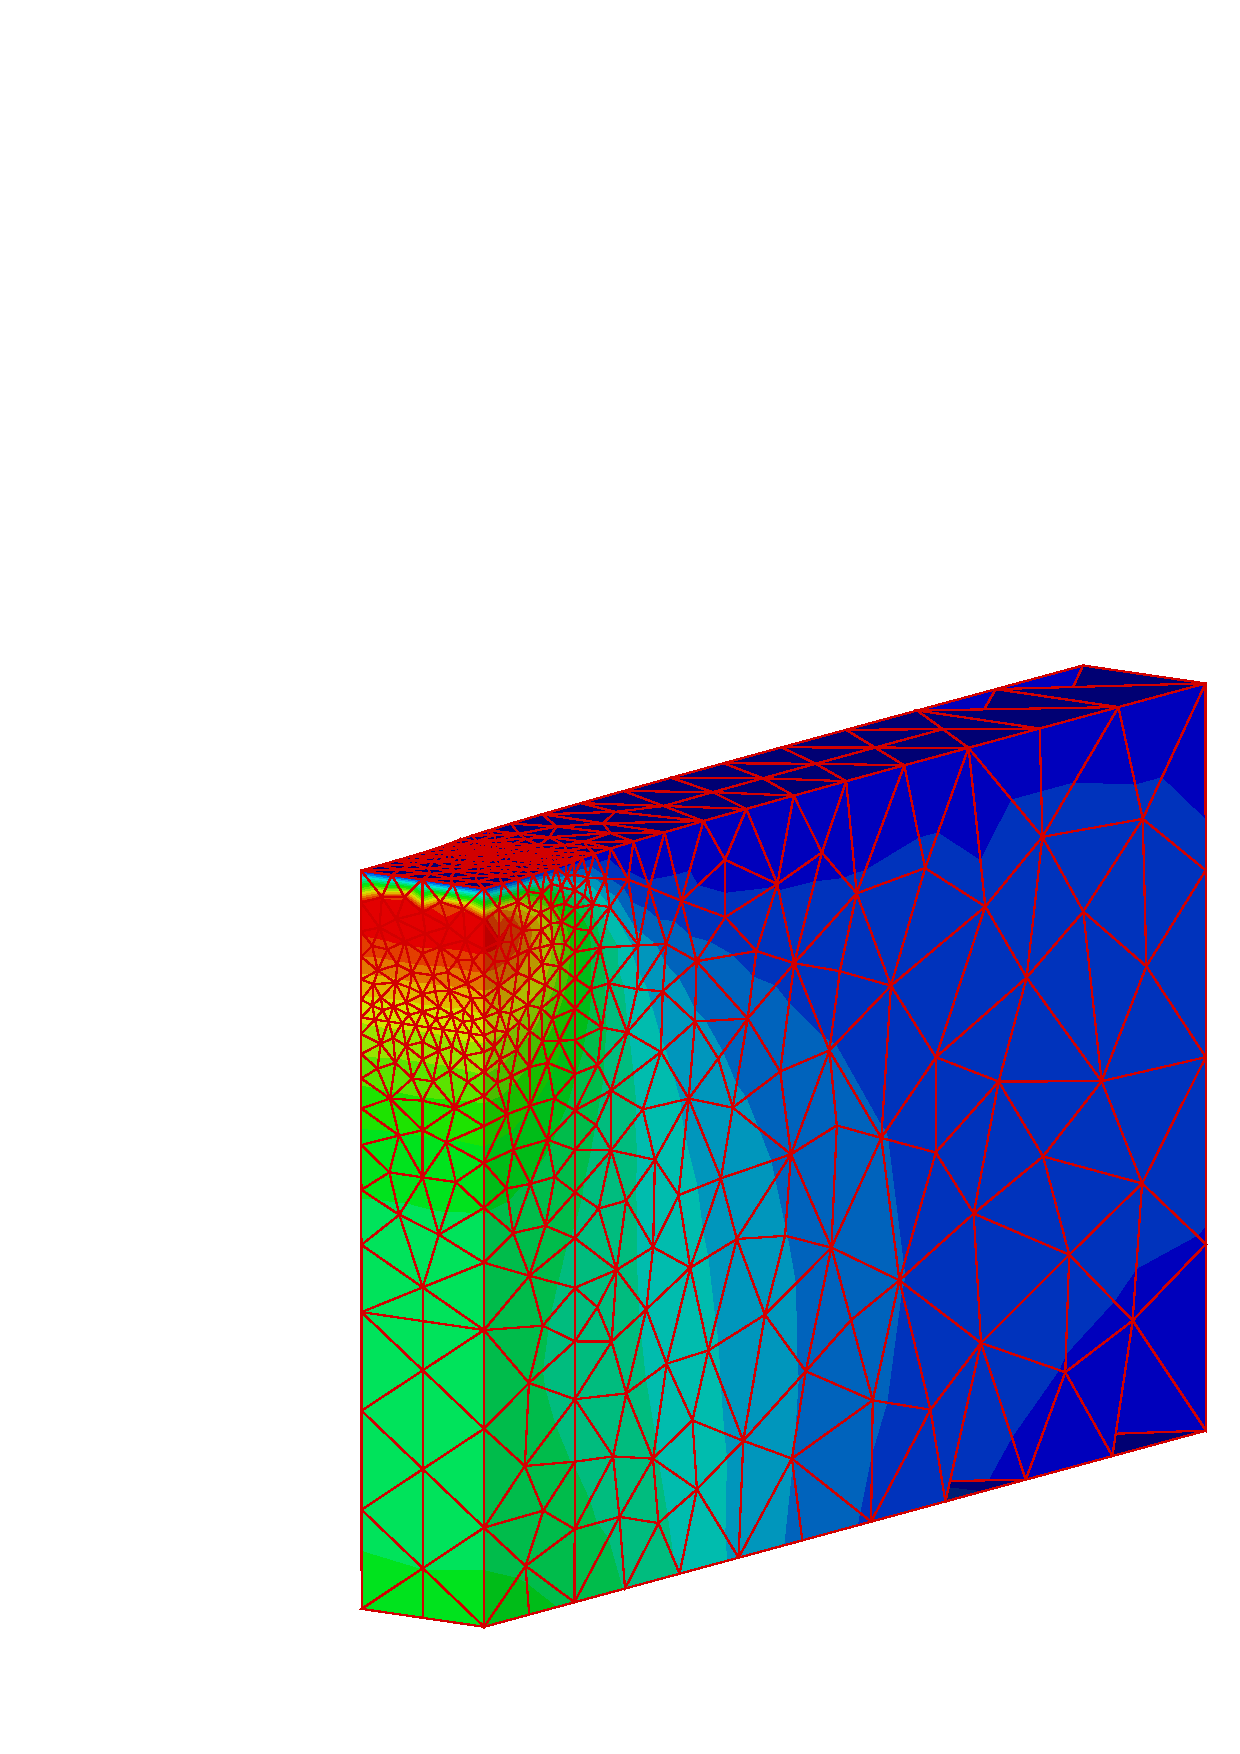
\includegraphics[width=0.44\textwidth]{chapter_14/figures/fig_14_1_4_b}
\end{center}
\vspace{-0.5cm}
\caption{Mesh geometry.}
\label{fig_HM3}
%\vspace{-1.0cm}
\end{figure}

\begin{figure}[!tbh]
\begin{center}
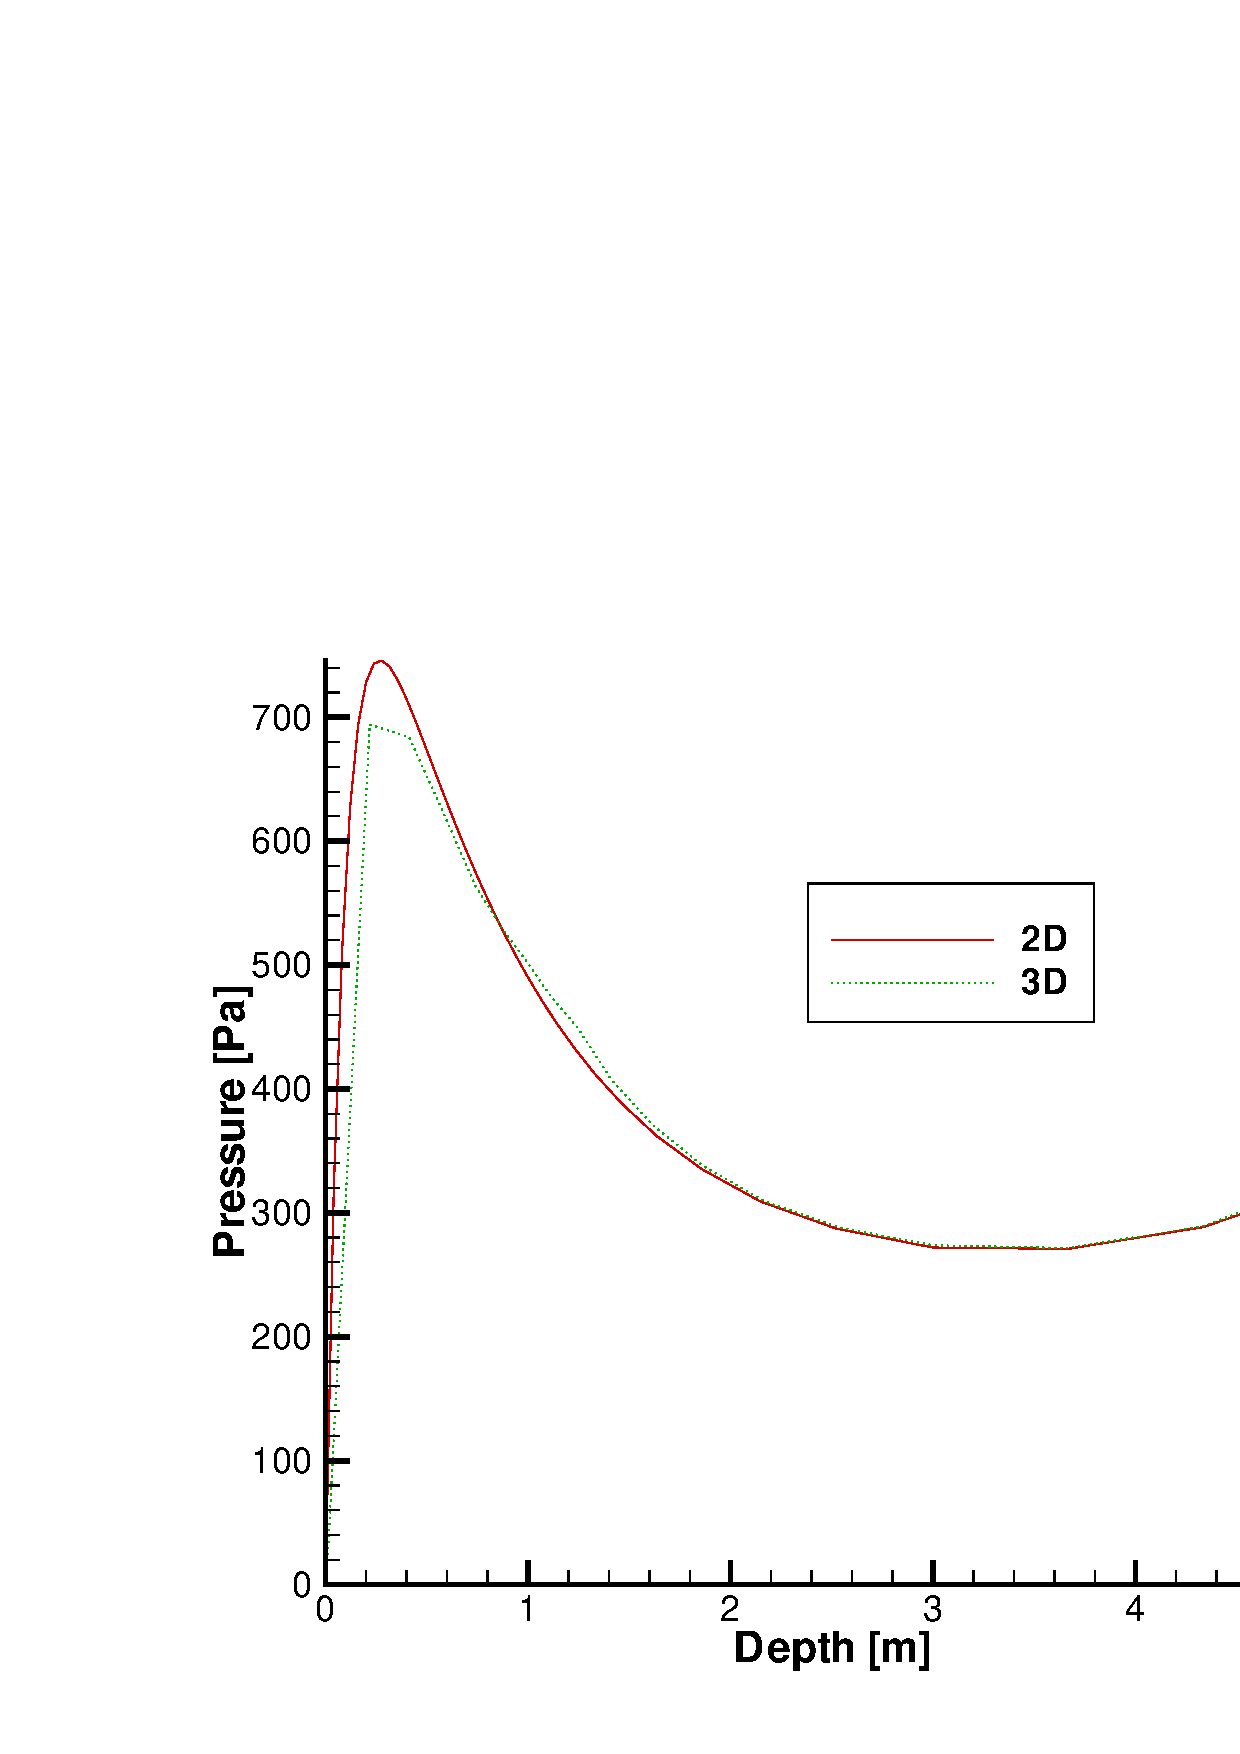
\includegraphics[width=0.49\textwidth]{chapter_14/figures/fig_14_1_5_a}
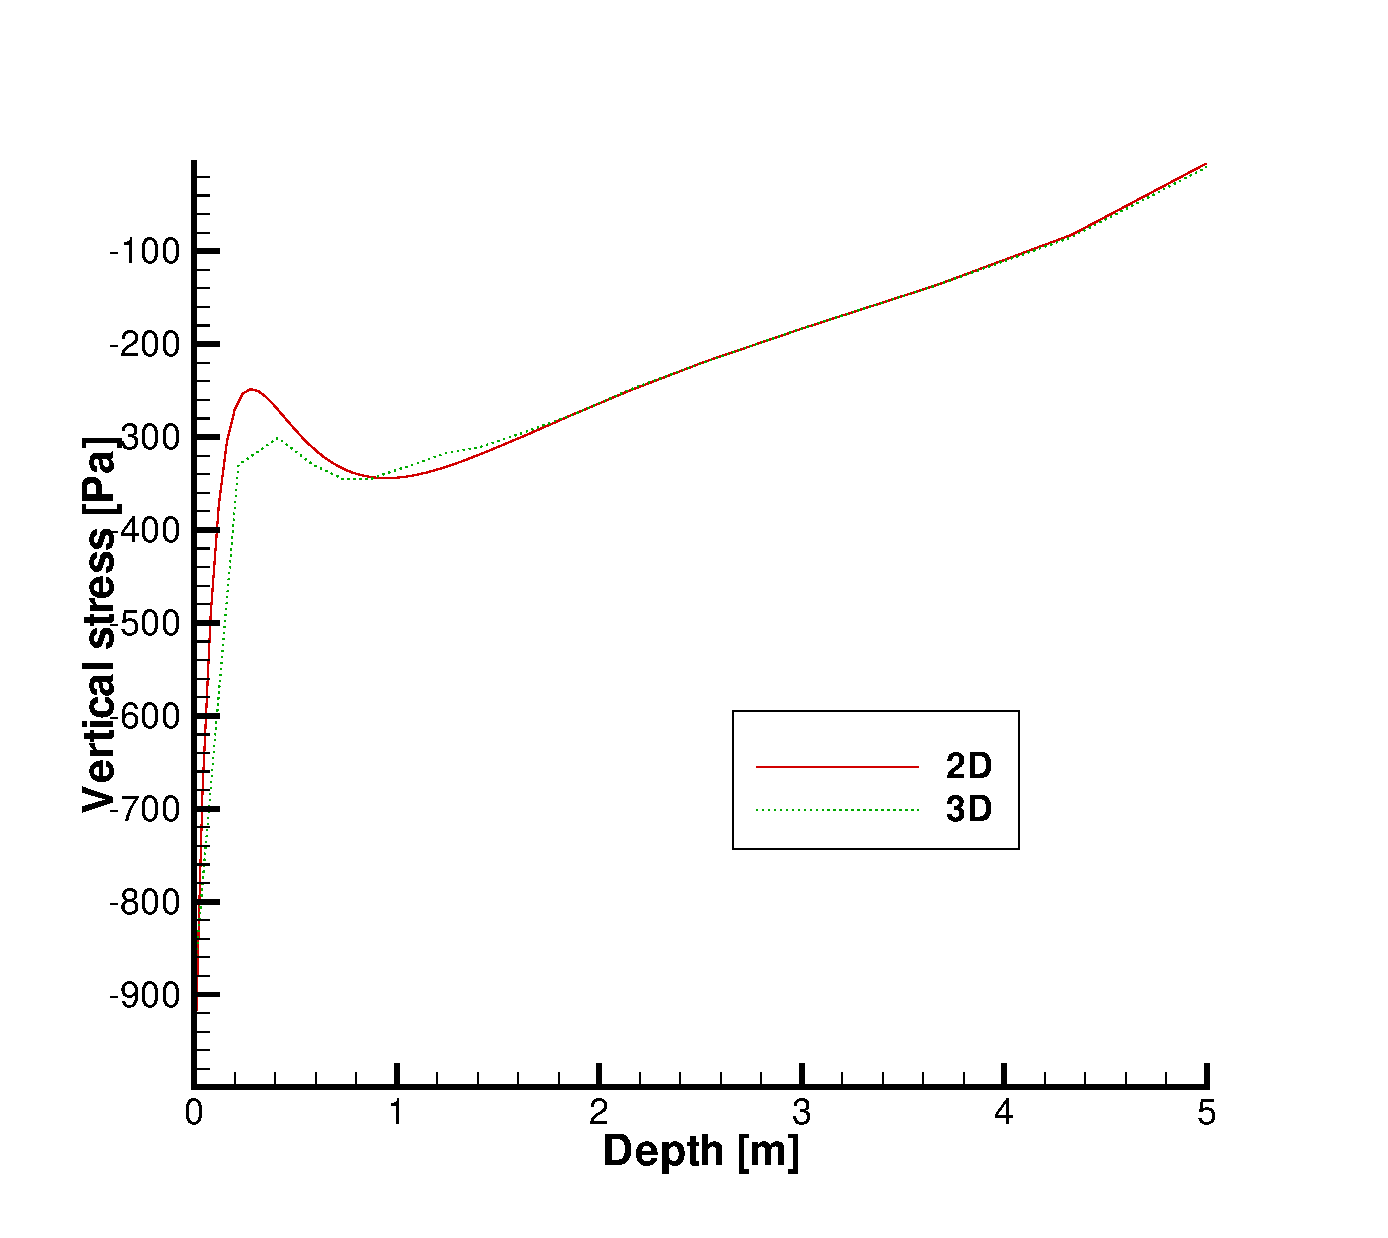
\includegraphics[width=0.49\textwidth]{chapter_14/figures/fig_14_1_5_b}
\end{center}
\caption{Comparison along symmetric axis.}  
\label{fig:e11}
\end{figure}

\begin{figure}[!tbh]
\begin{center}
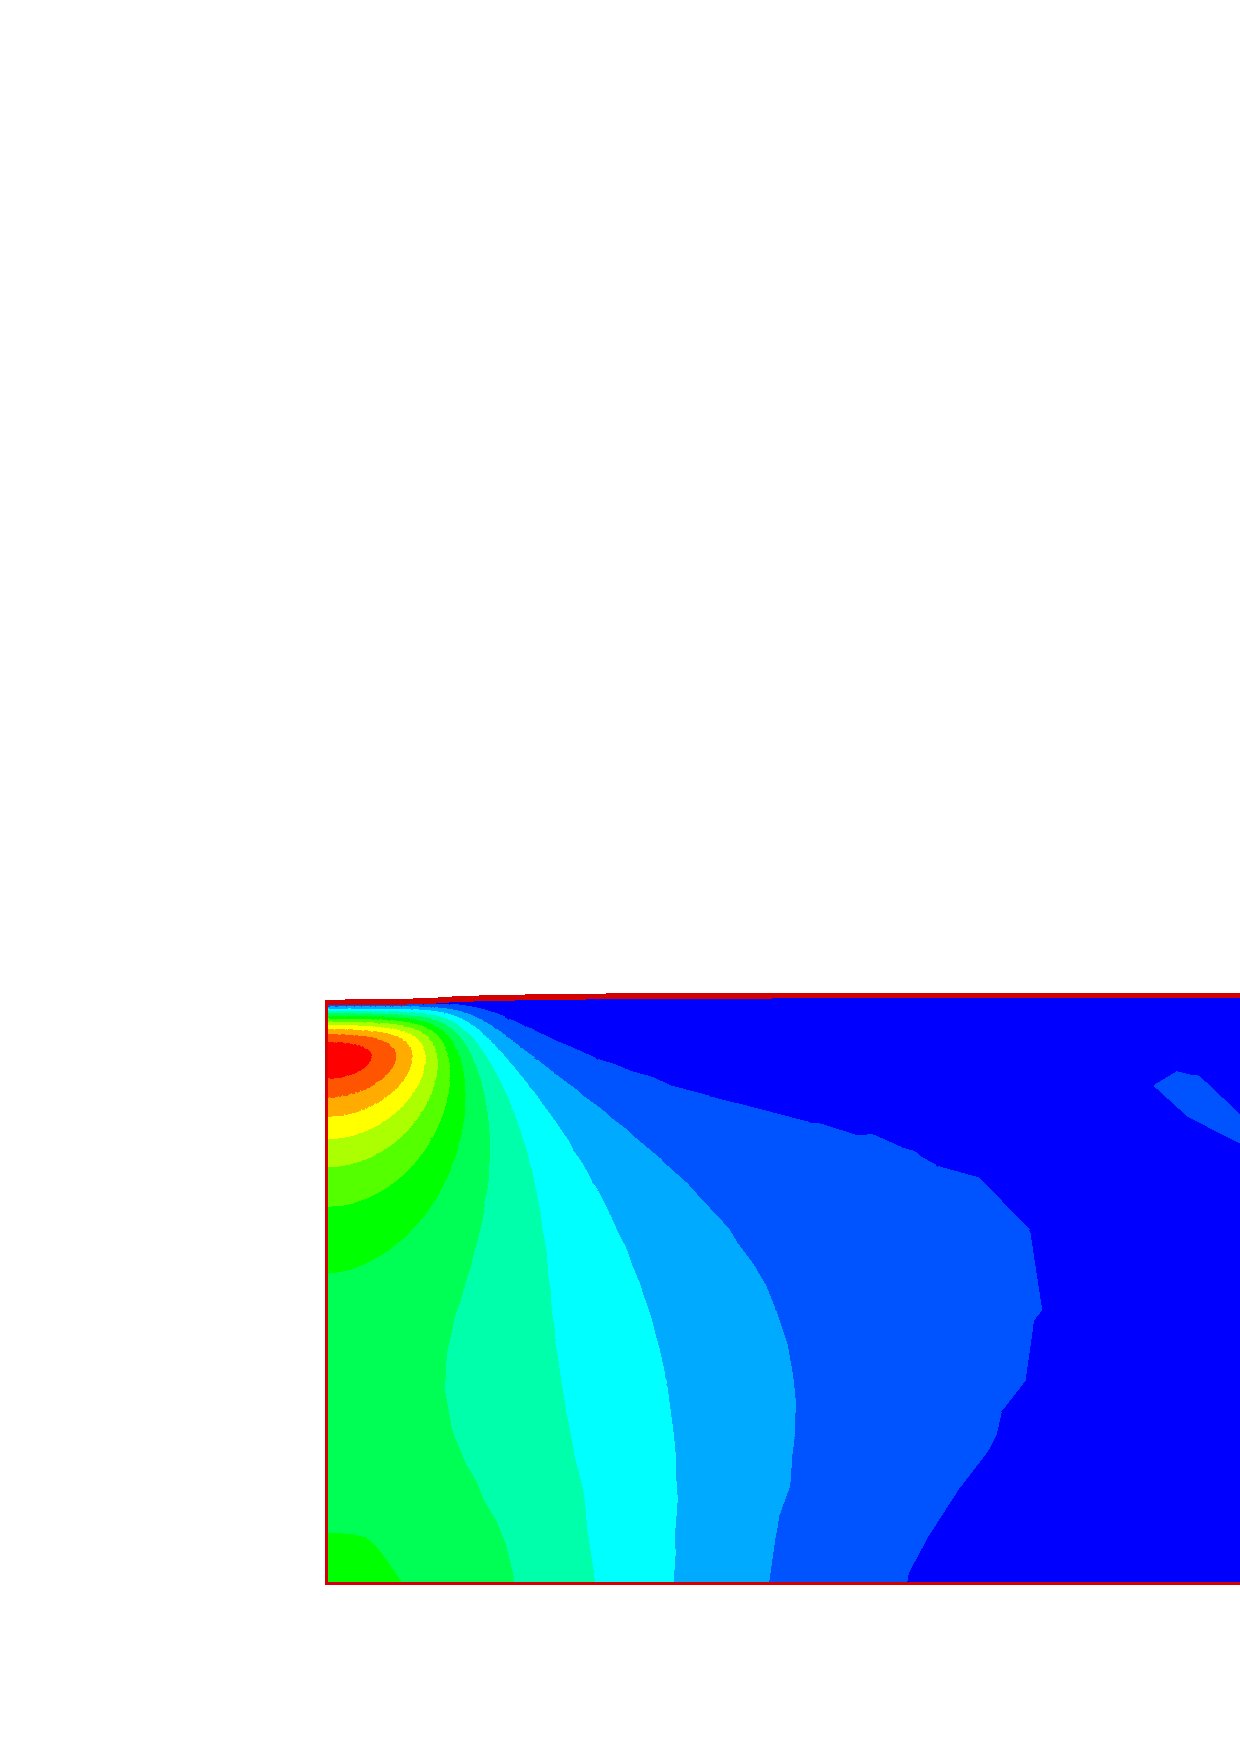
\includegraphics[width=0.49\textwidth]{chapter_14/figures/fig_14_1_6_a}
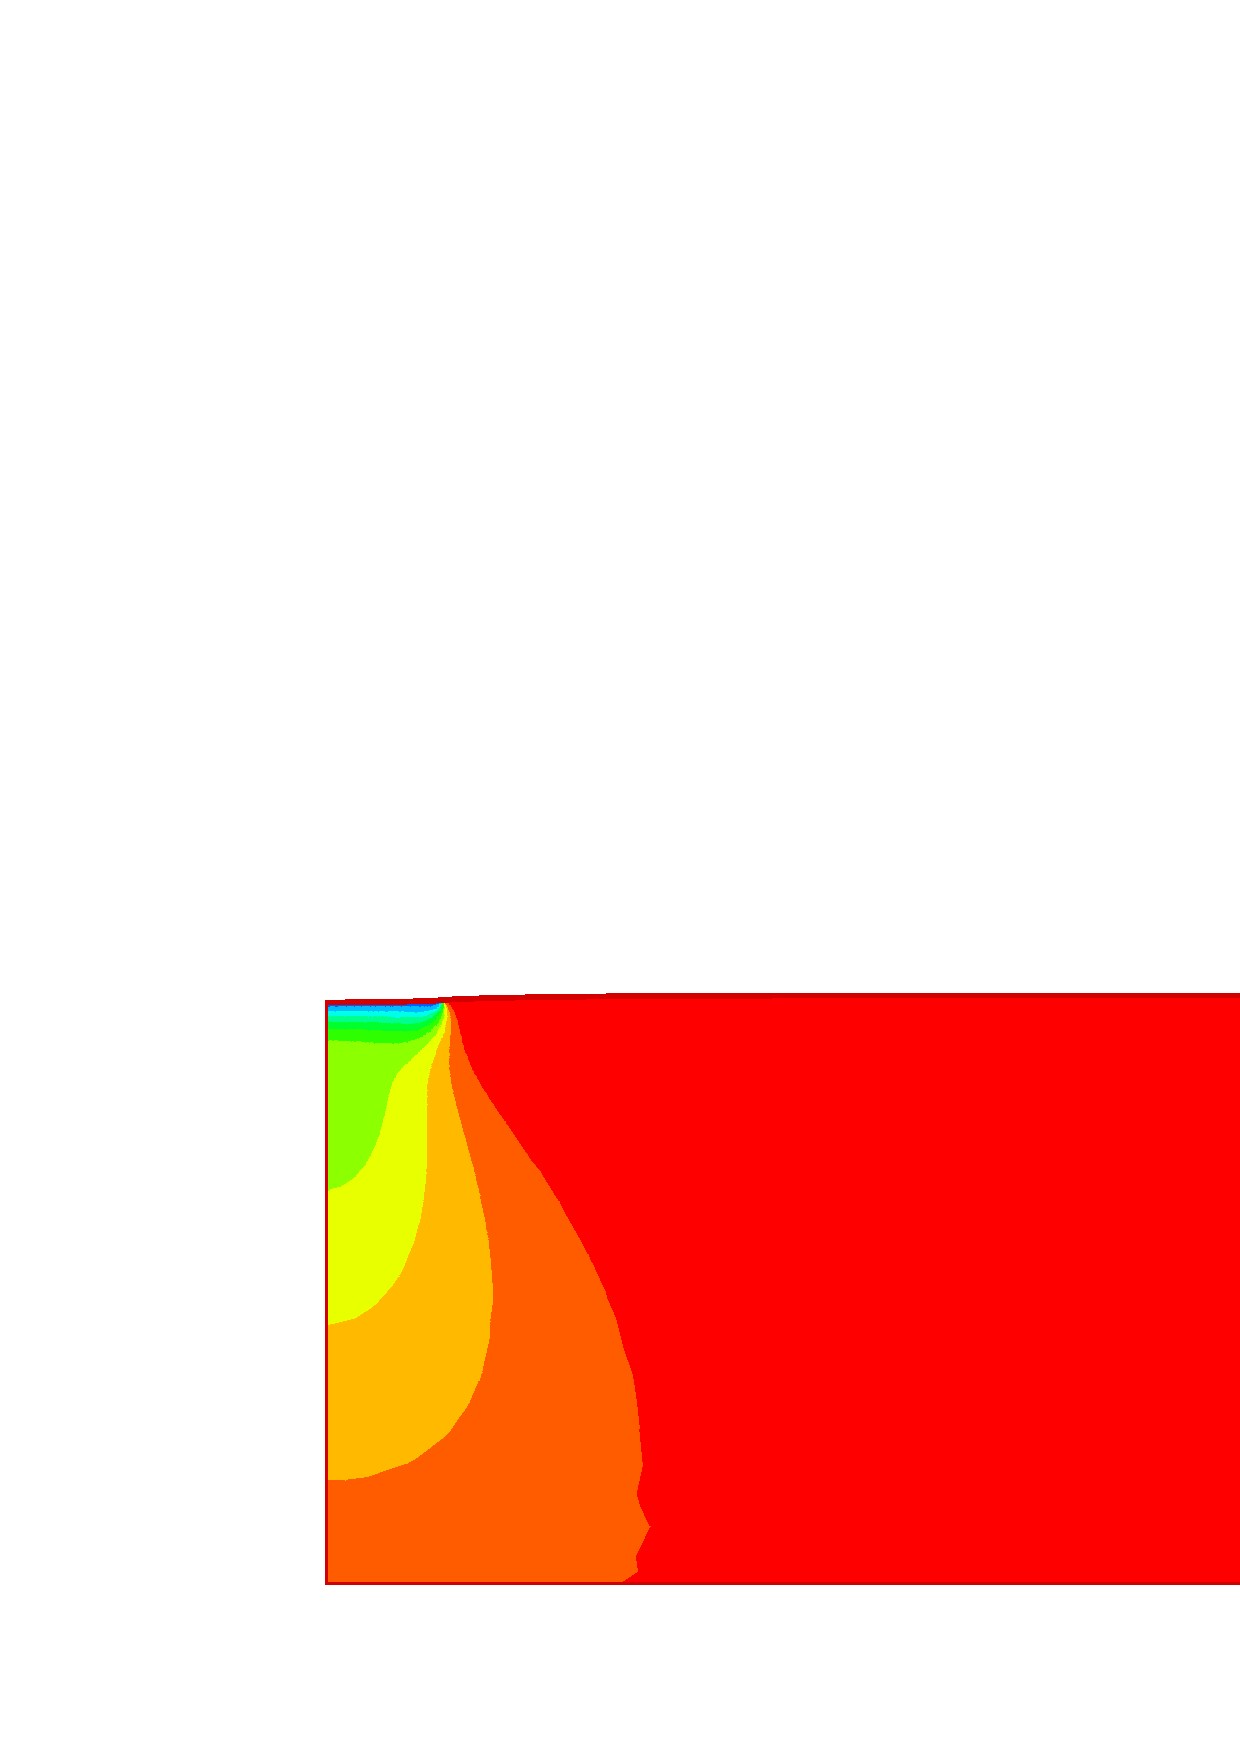
\includegraphics[width=0.49\textwidth]{chapter_14/figures/fig_14_1_6_b}
\end{center}
\vspace{-0.5cm}
\caption{2D contours.}
\label{fig:e10}

\begin{center}
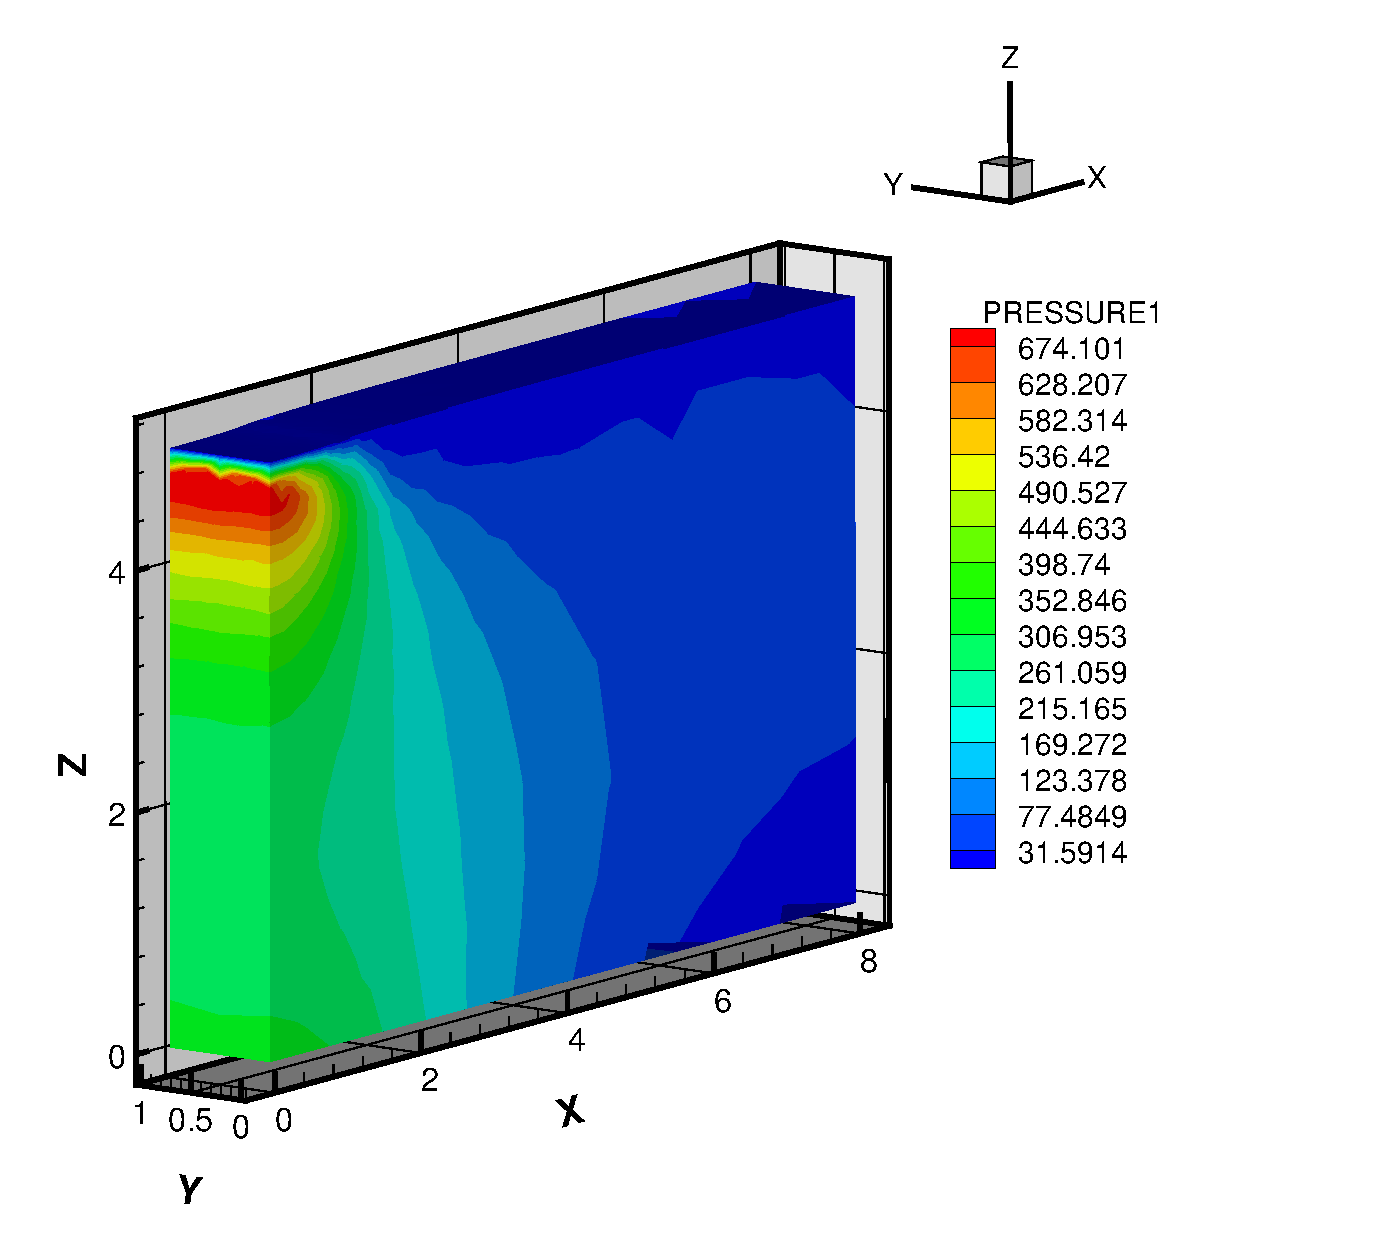
\includegraphics[width=0.49\textwidth]{chapter_14/figures/fig_14_1_7_a}
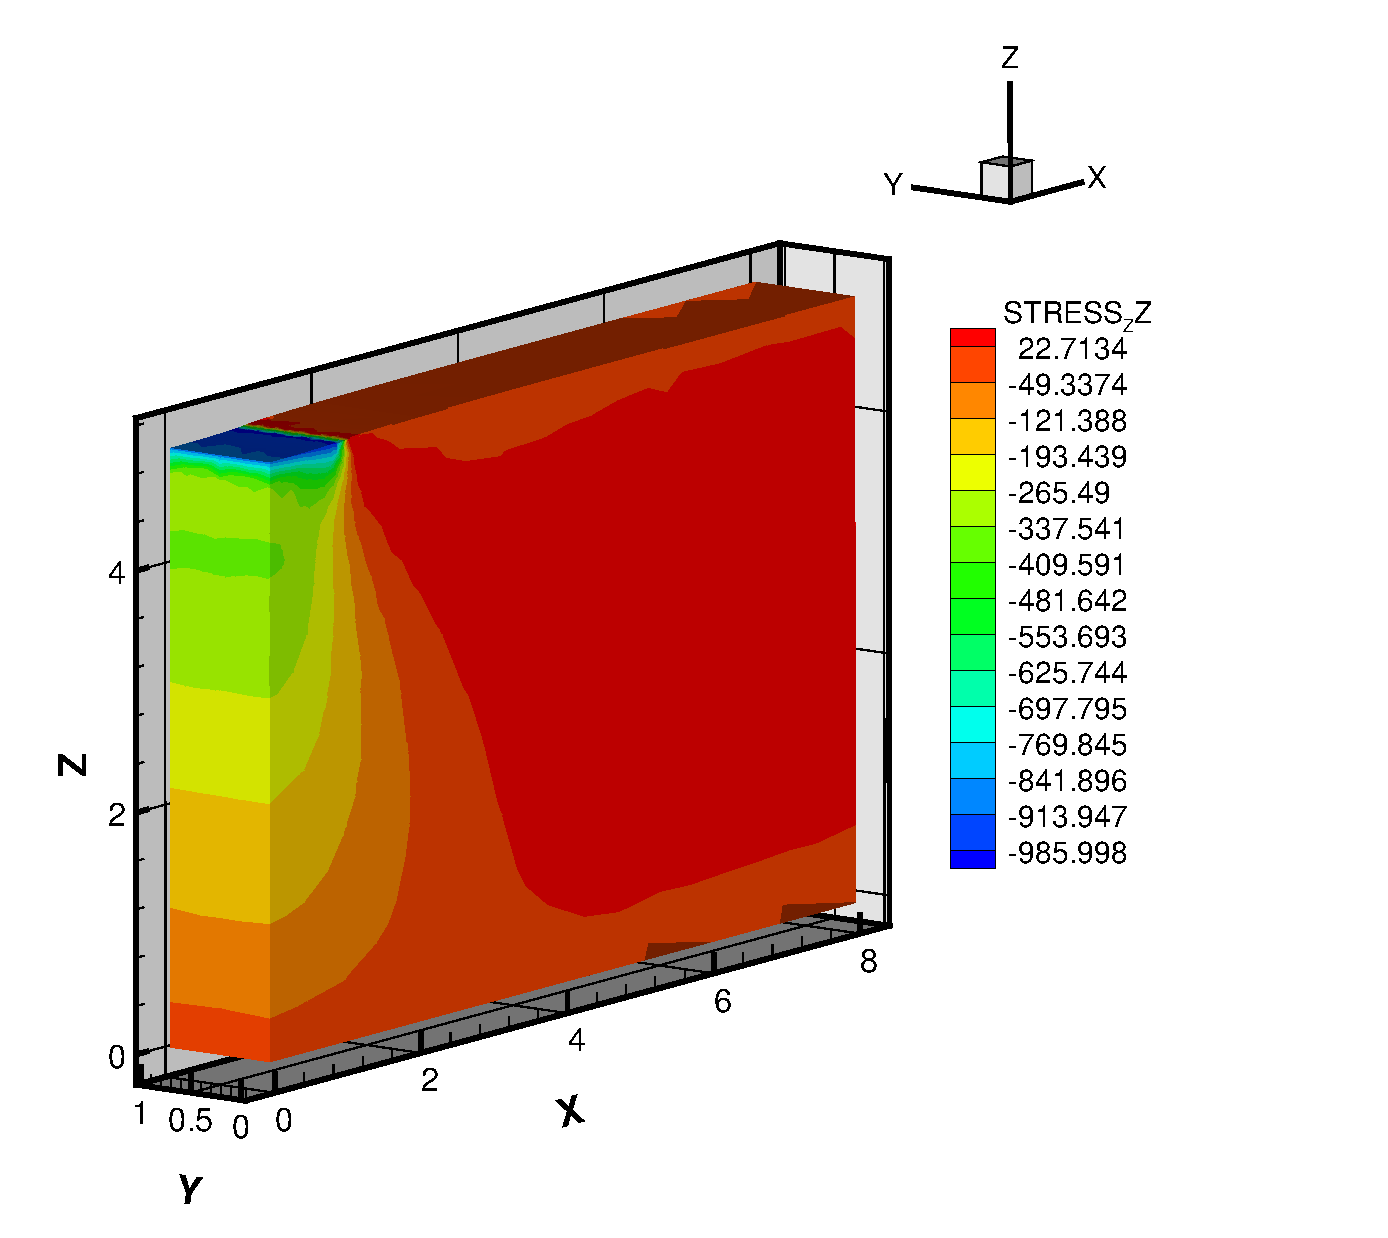
\includegraphics[width=0.49\textwidth]{chapter_14/figures/fig_14_1_7_b}
\end{center}
\vspace{-0.5cm}
\caption{3D contours.}
\label{fig:e12}
\end{figure}
\subsection{Distributed footing: Poroelastic cube (3D) with dynamic consolidation}
Considering the same problem design as the previous section, the mechanical calculation is now extended to allow for time-dependent deformation. In other words, solid displacements are no longer solved to equilibrium, so that solid velocity may be non-zero following solution of the mechanical system.

\subsubsection*{Definition}
All stresses and pressure are zero at the beginning of deformation. Strip
loading ($\sigma_{yy}=\sigma_0$ in $x\in[0,1]$), zero stresses
($\sigma_{yy}=\sigma_{xy}=0$ in $x\in(1,8]$) and zero pressure at
the top; no horizontal flux, no horizontal displacements and zero
shear stresses at left and right hand sides; no vertical flux and no
displacements at bottom (Figure \ref{fig-setting}).

Material parameters are given in Table \ref{tab:mat-dynam}.

\begin{table}[!htb]
\begin{center}
\begin{tabular}{lll}
\hline{\smallskip}
Property & Value & Unit \\
\hline
Young's modulus & $3\times 10^{4}$  & $N/m^{2}$ \\
Poisson's ratio & $0.2, 0.4$       & $-$ \\
Permeability    & $10^{-10}$        & $m^2$ \\
Fluid viscosity & $10^{-3}$         & $Pa\,s$ \\
\hline
\end{tabular}
\end{center}
\caption{Material properties of dynamic consolidation problem.}
\label{tab:mat-dynam}
\end{table}

\subsubsection*{Results}
Time duration is ten time steps. The following figures, Fig. \ref{fig_dynHM1}--\ref{fig_dynHM4} show the distribution of state variables within the domain after 10 time steps. Such distribution is similar to the static case illustrated in Fig. \ref{fig:e10}.
 
\begin{figure}[!htb]
\begin{center}
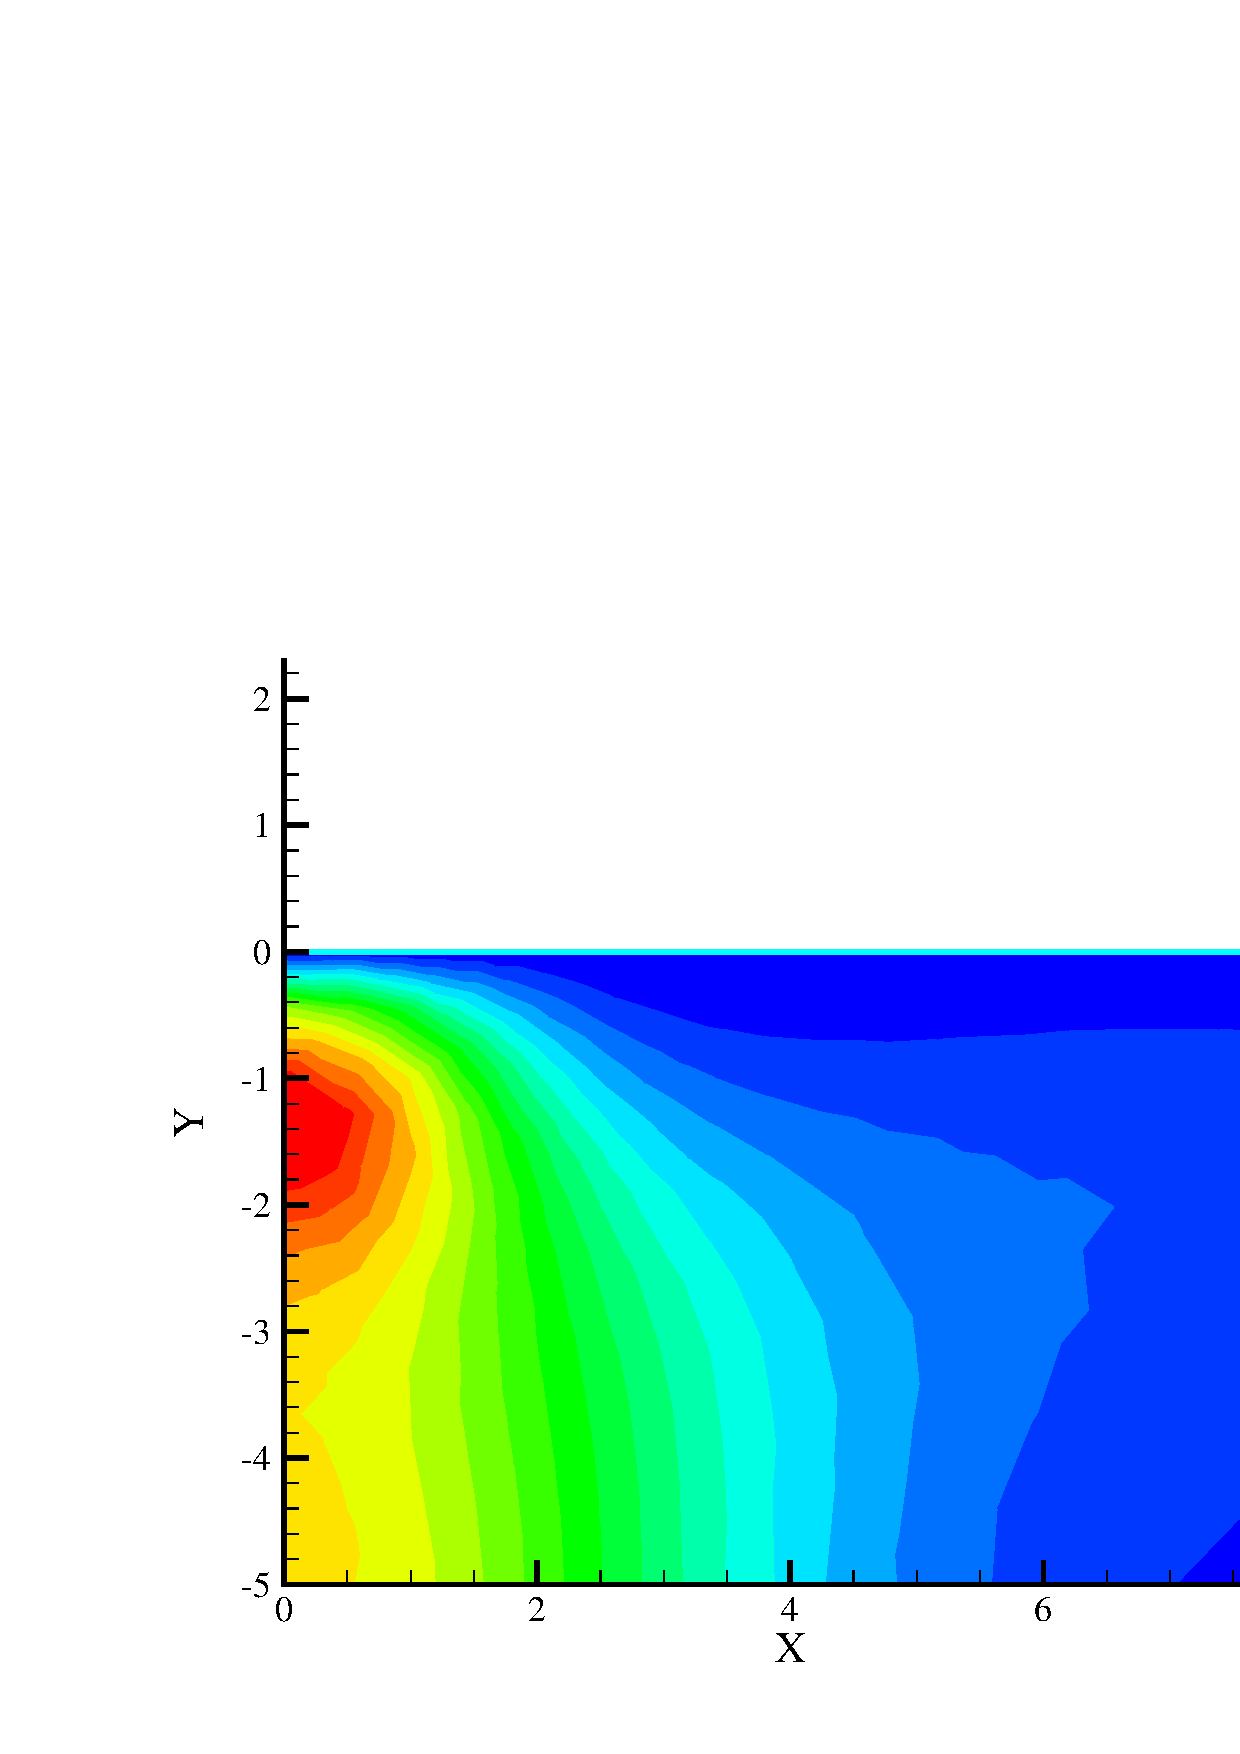
\includegraphics[width=0.49\textwidth]{chapter_14/figures/fig_14_1_8_a}
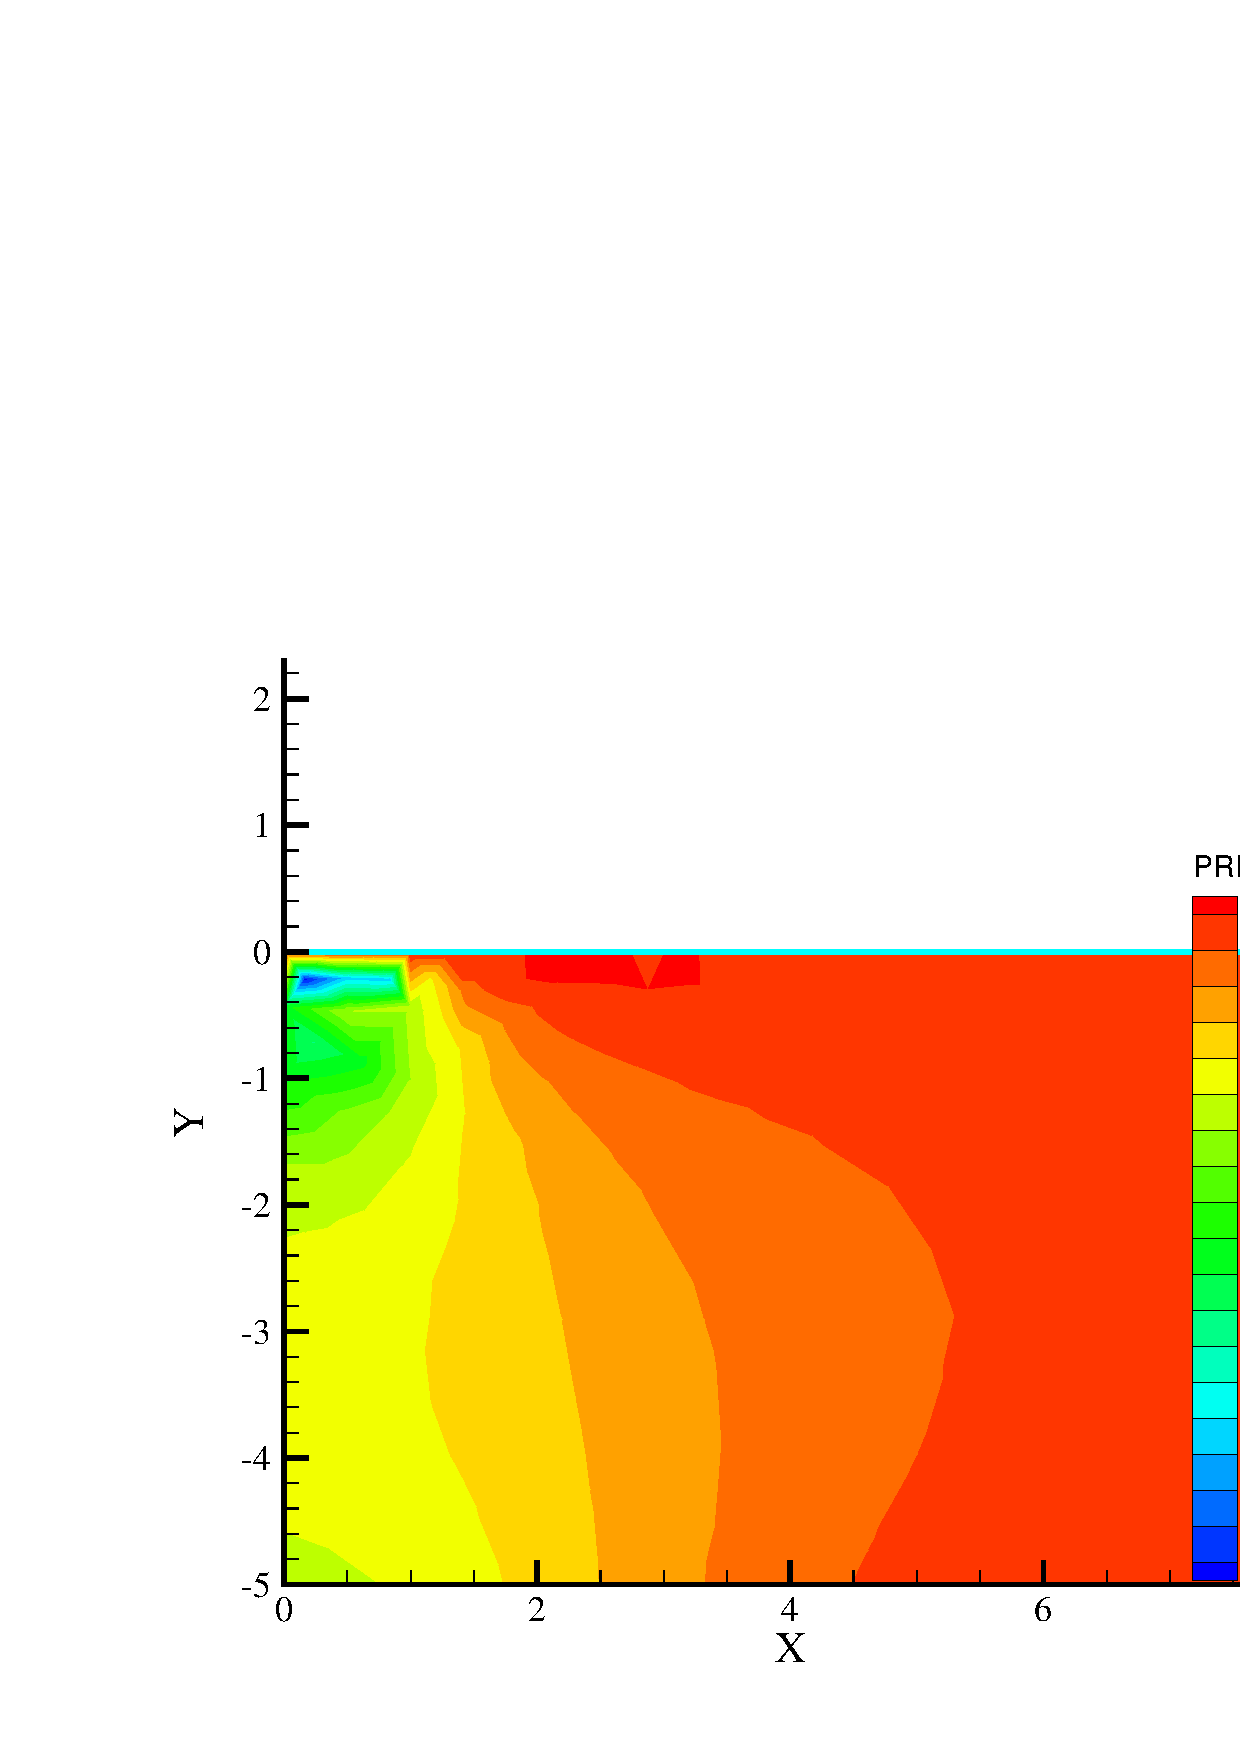
\includegraphics[width=0.49\textwidth]{chapter_14/figures/fig_14_1_8_b}
\end{center}
\caption{Fluid pressures $p$ and rate of fluid pressure $\dot p$ }
\label{fig_dynHM1}
\end{figure}

\begin{figure}[!htb]
\begin{center}
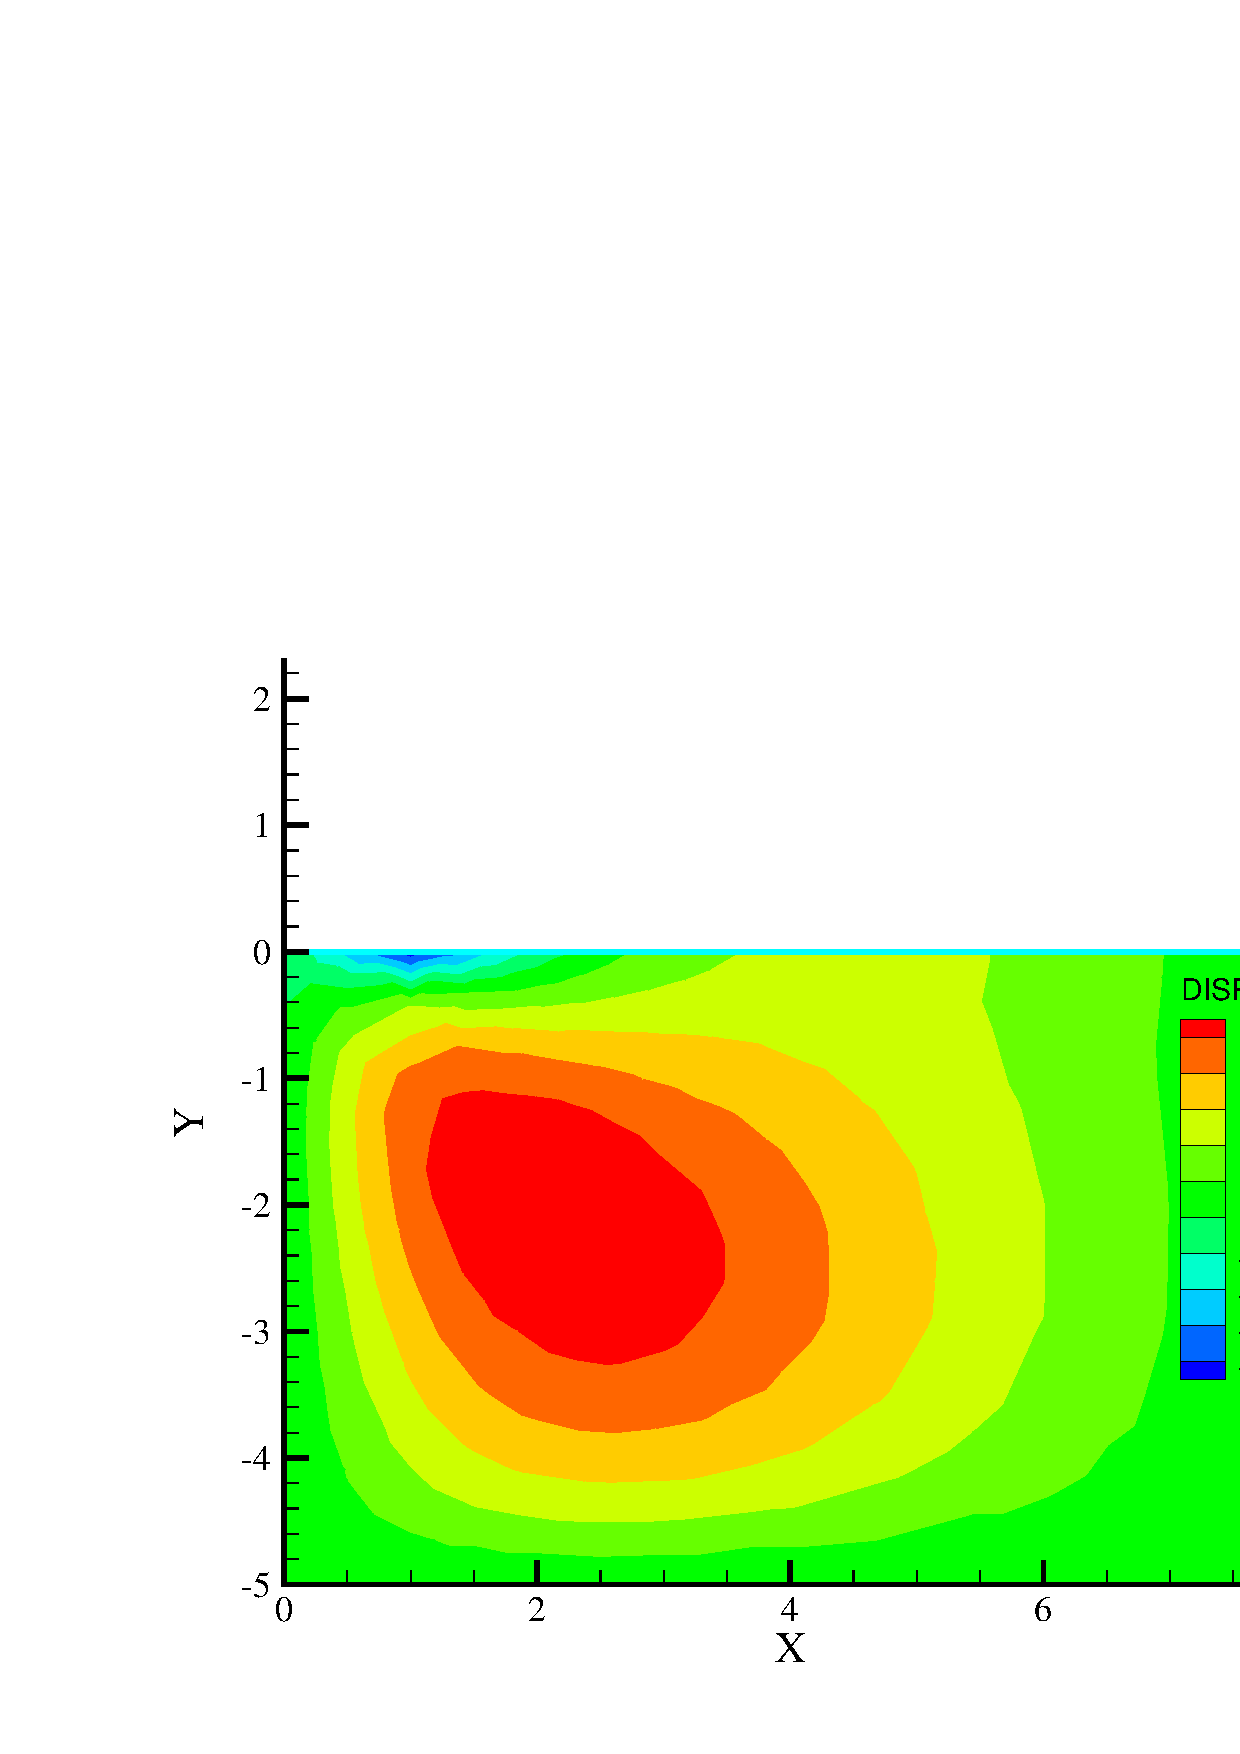
\includegraphics[width=0.32\textwidth]{chapter_14/figures/fig_14_1_9_a}
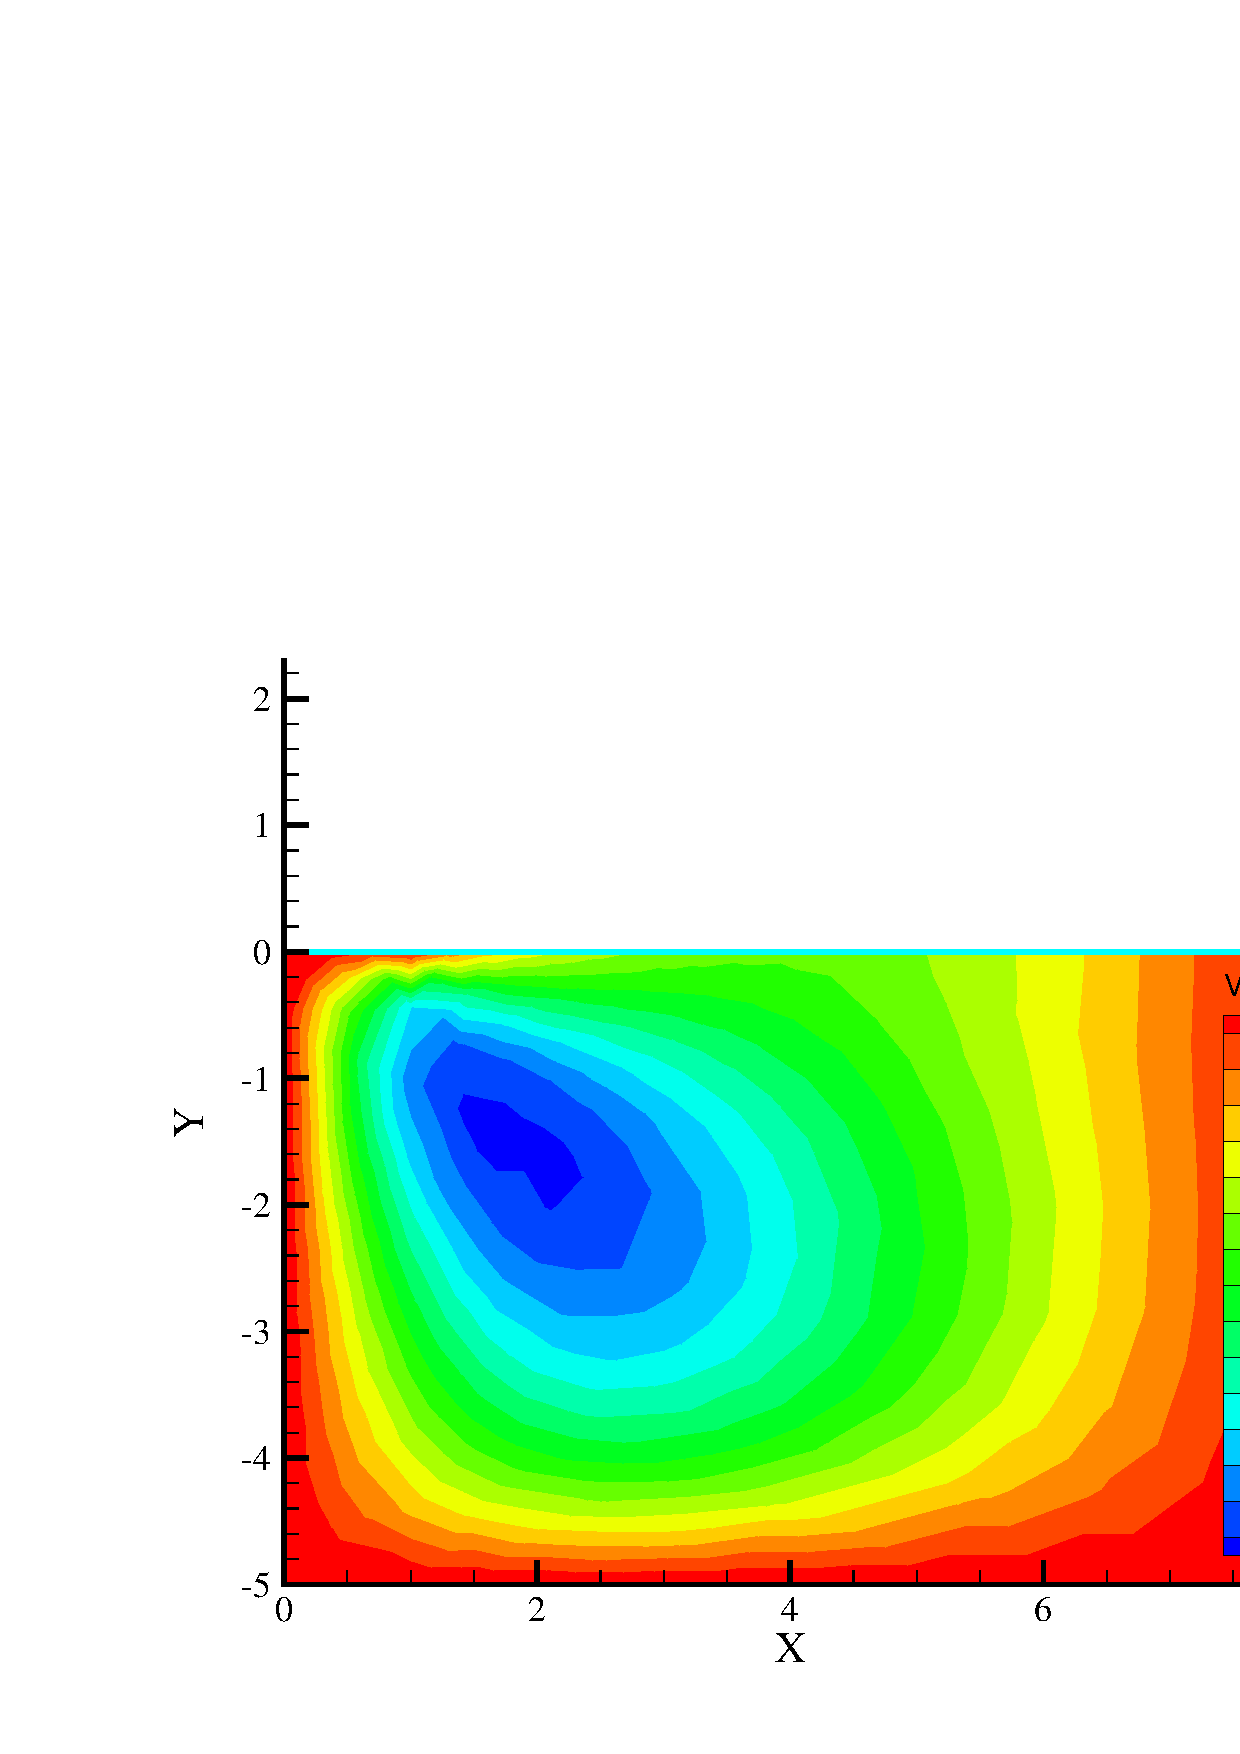
\includegraphics[width=0.32\textwidth]{chapter_14/figures/fig_14_1_9_b}
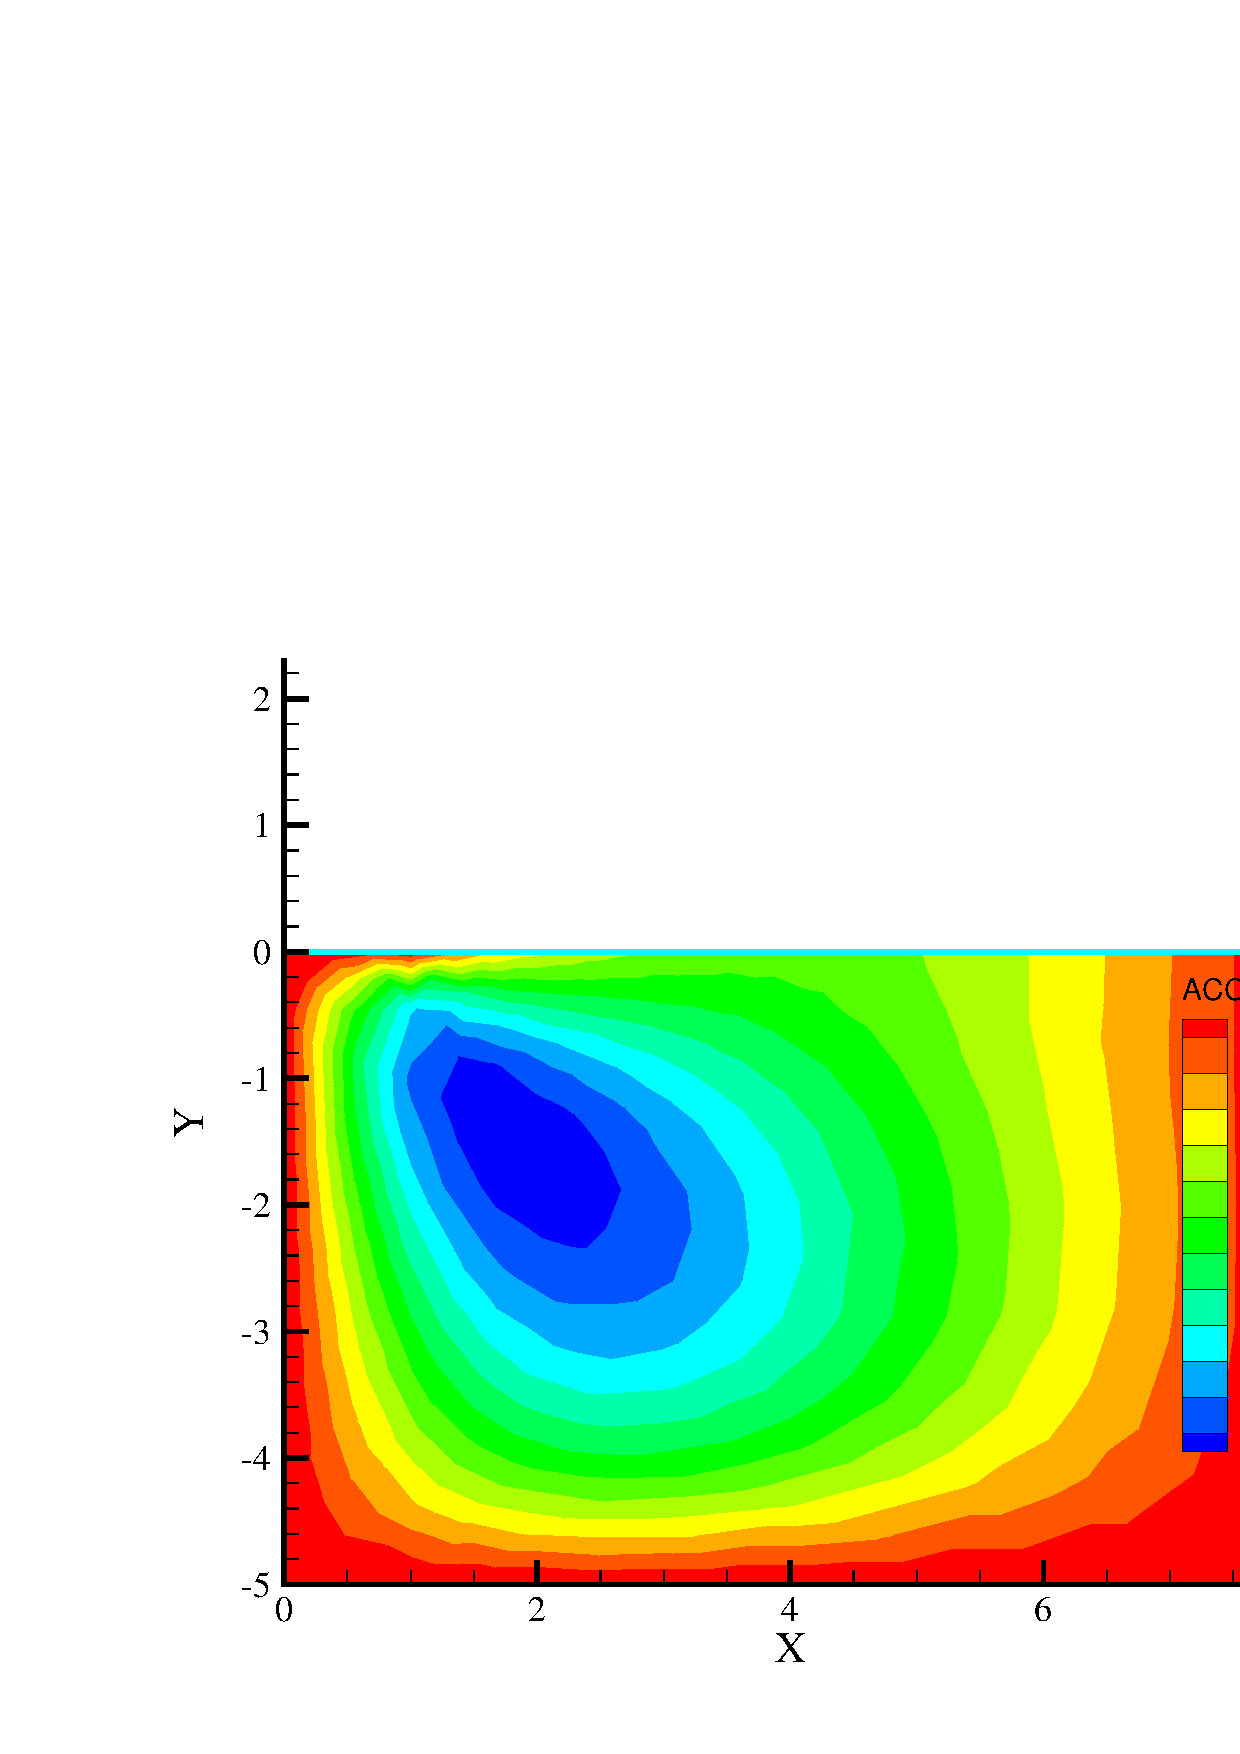
\includegraphics[width=0.32\textwidth]{chapter_14/figures/fig_14_1_9_c}
\end{center}
\caption{Displacement, its rate and acceleration: horizontal component}
\label{fig_dynHM2}
%\end{figure}
%\begin{figure}[!htb]
\begin{center}
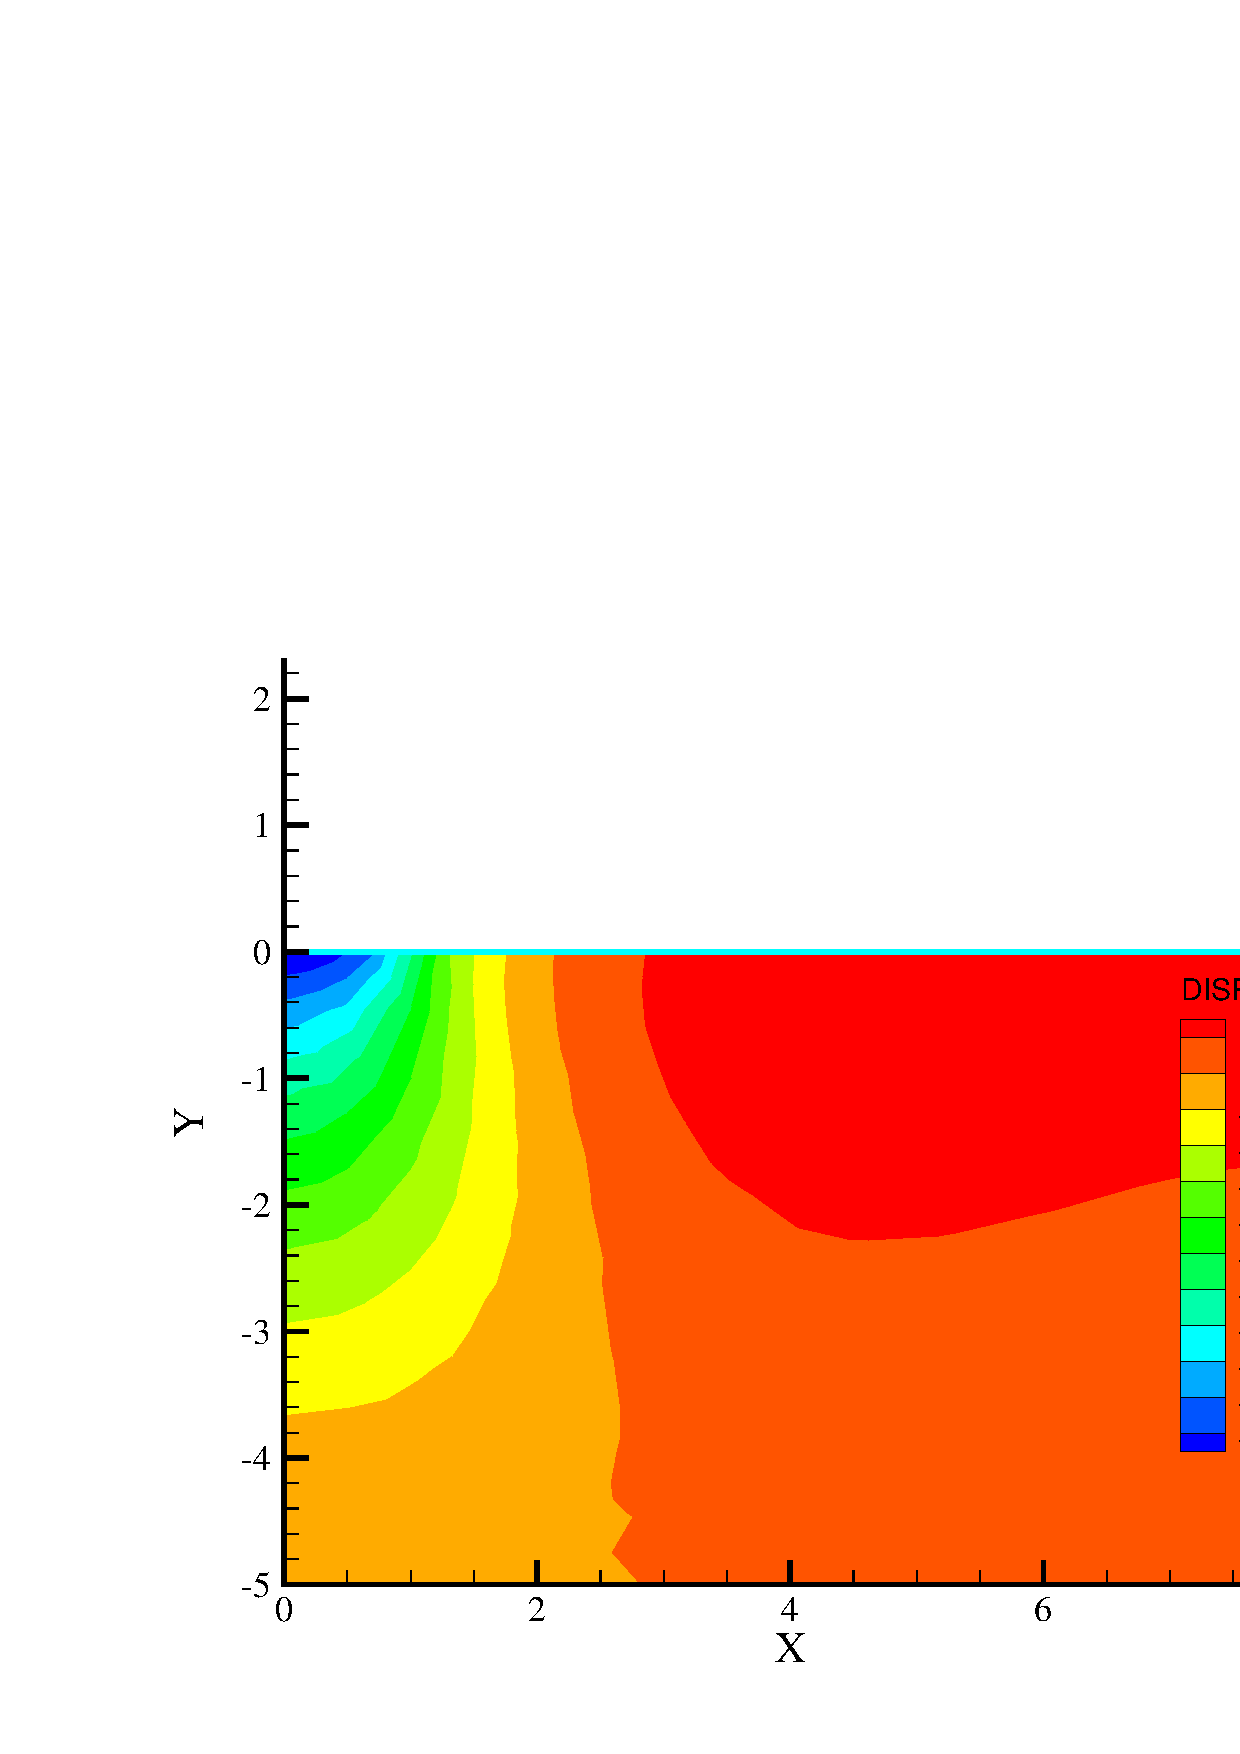
\includegraphics[width=0.32\textwidth]{chapter_14/figures/fig_14_1_10_a}
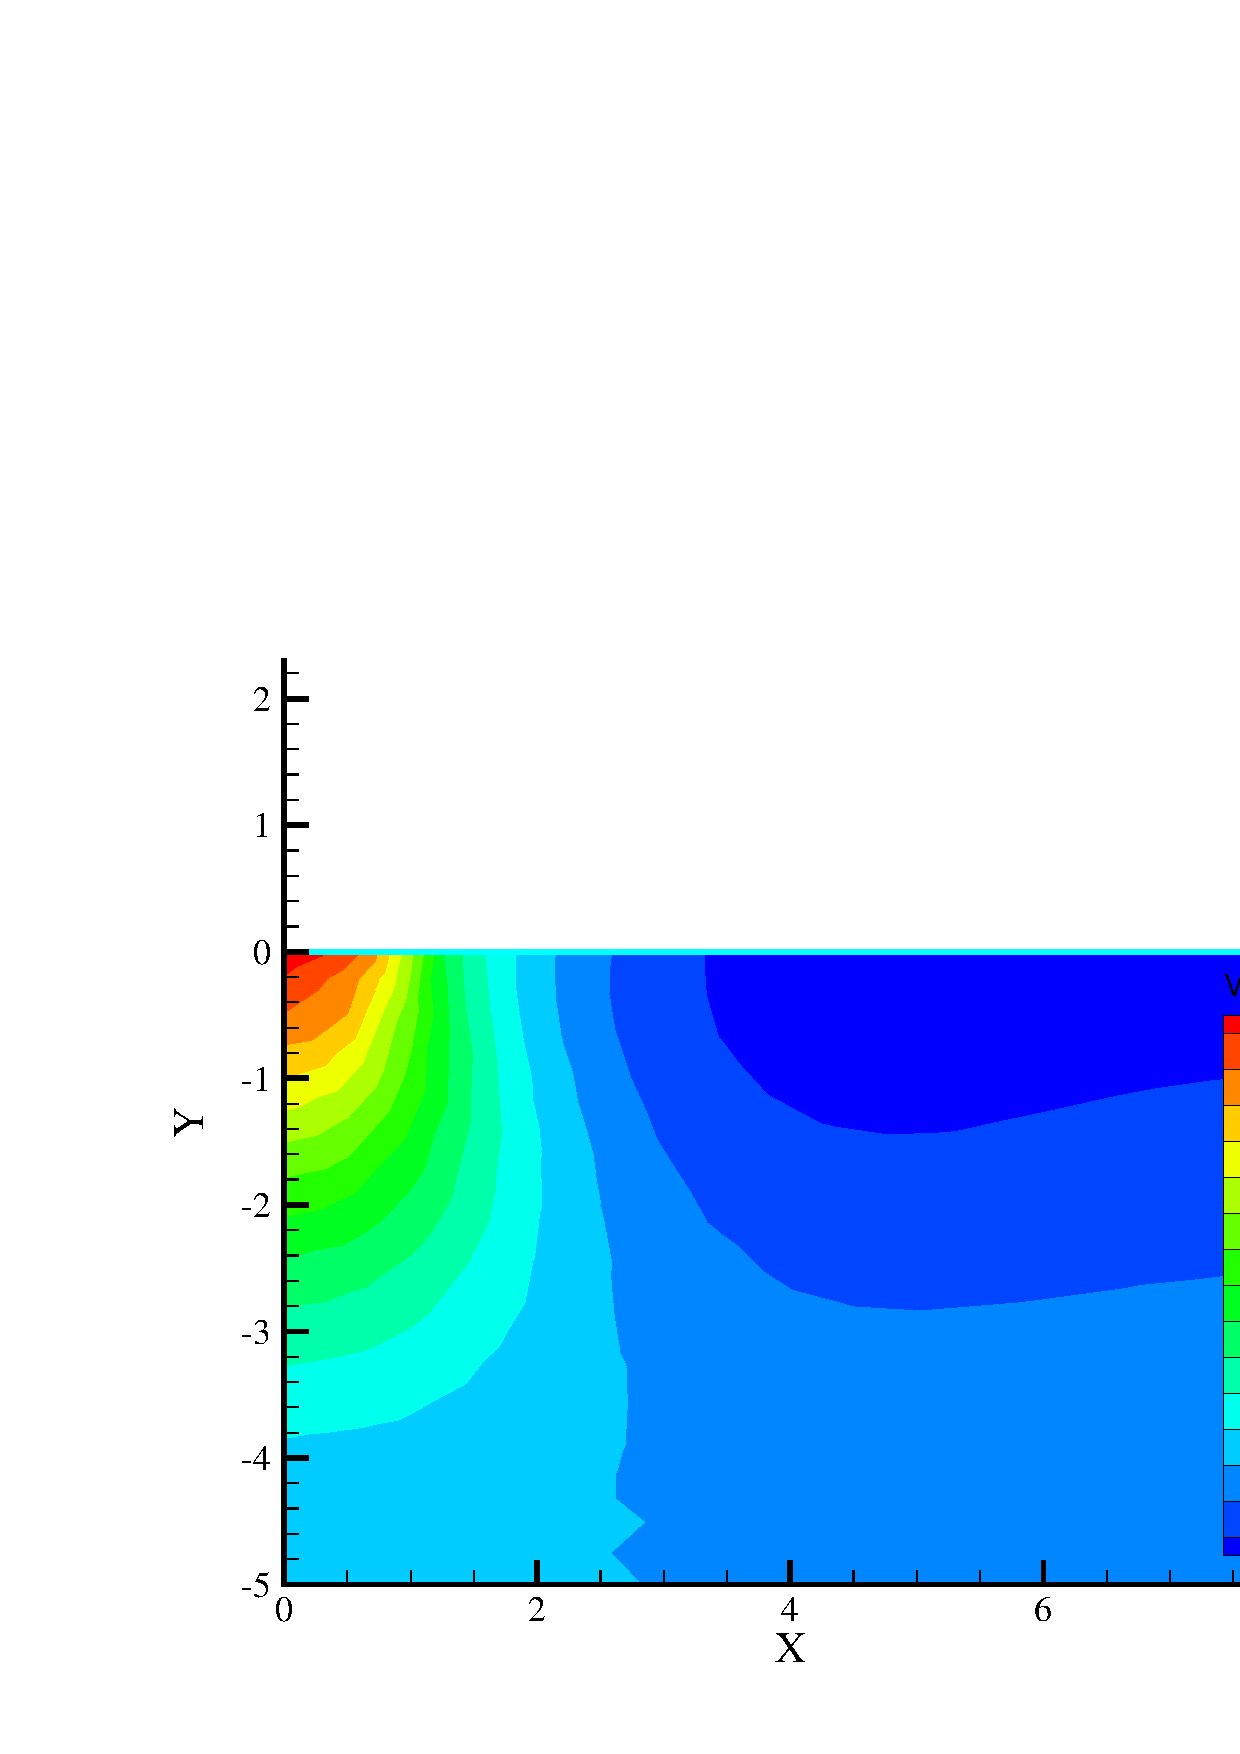
\includegraphics[width=0.32\textwidth]{chapter_14/figures/fig_14_1_10_b}
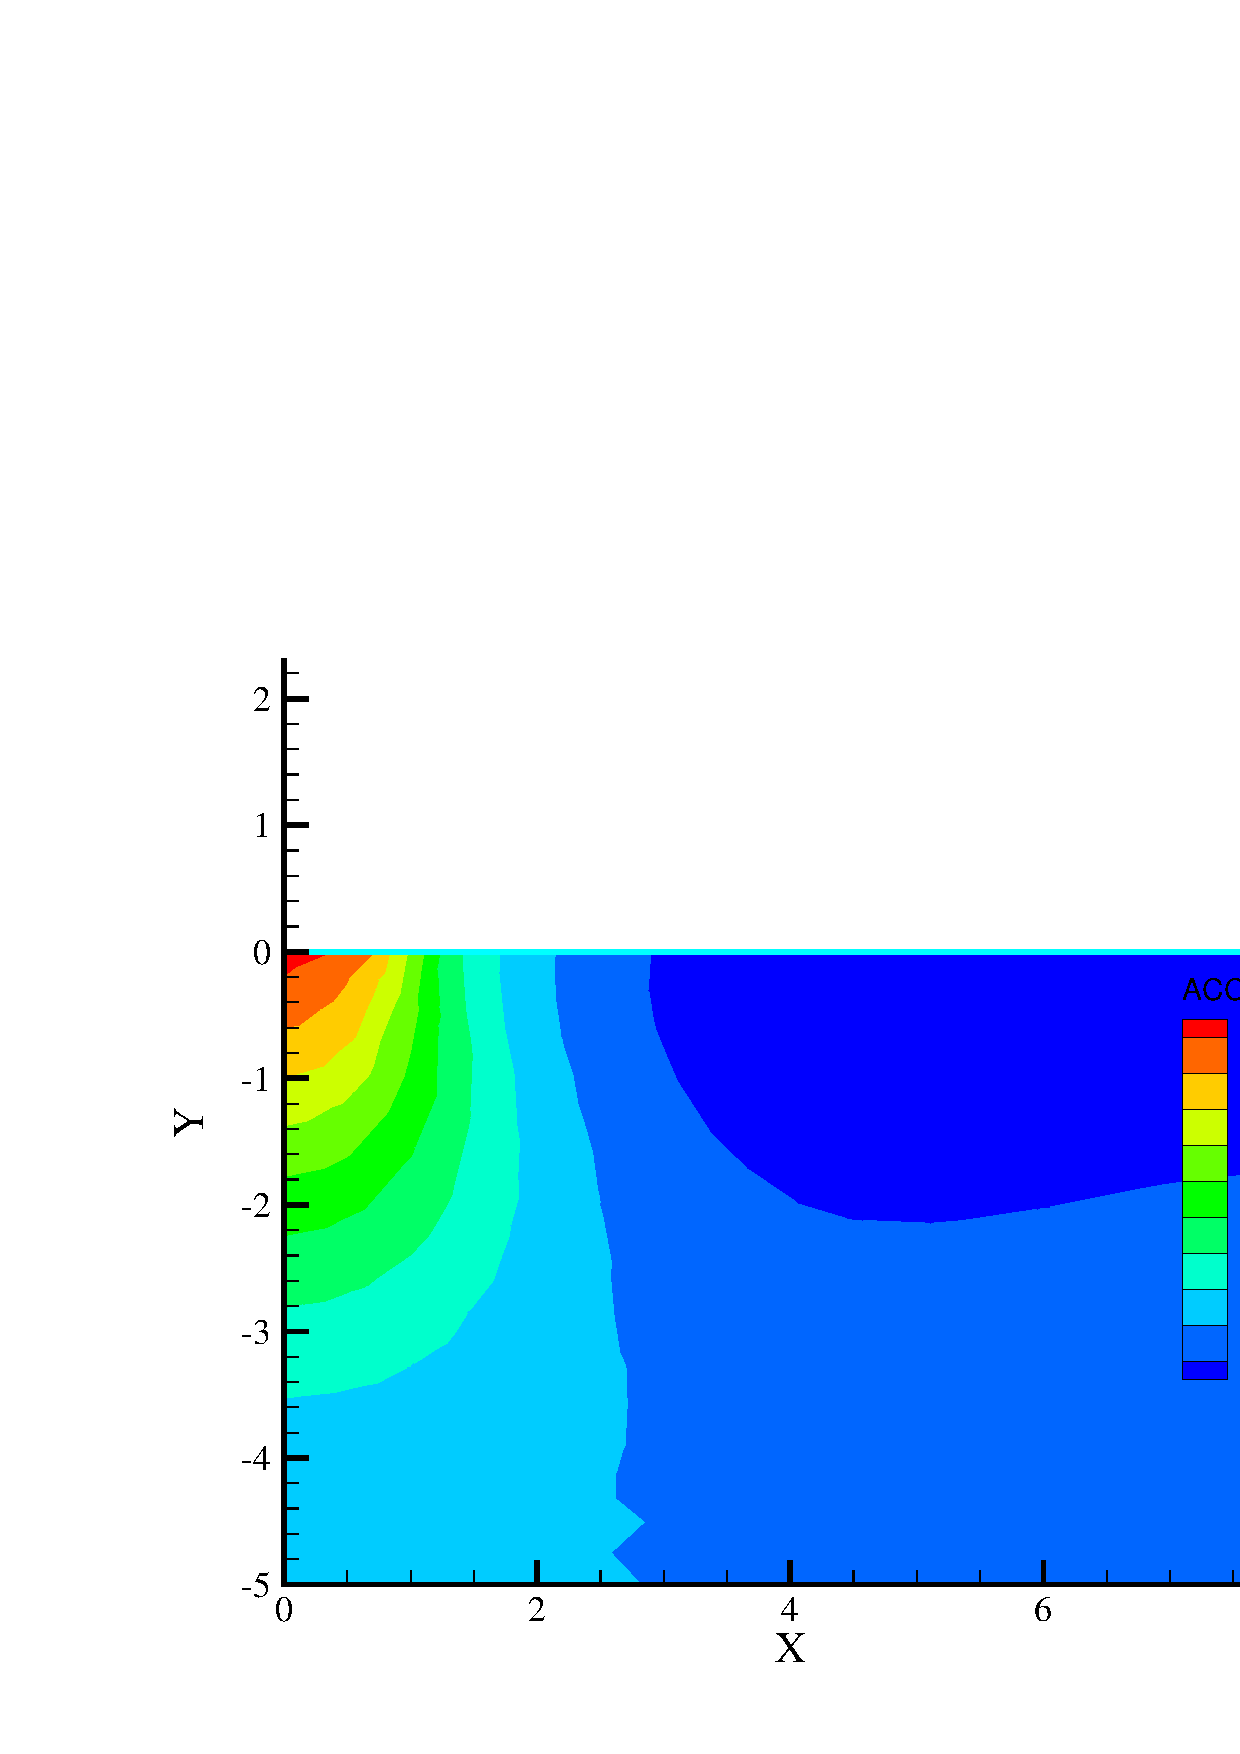
\includegraphics[width=0.32\textwidth]{chapter_14/figures/fig_14_1_10_c}
\end{center}
\caption{Displacement, its rate and acceleration: vertical component}
\label{fig_dynHM3}
\end{figure}
\begin{figure}[!htb]
\begin{center}
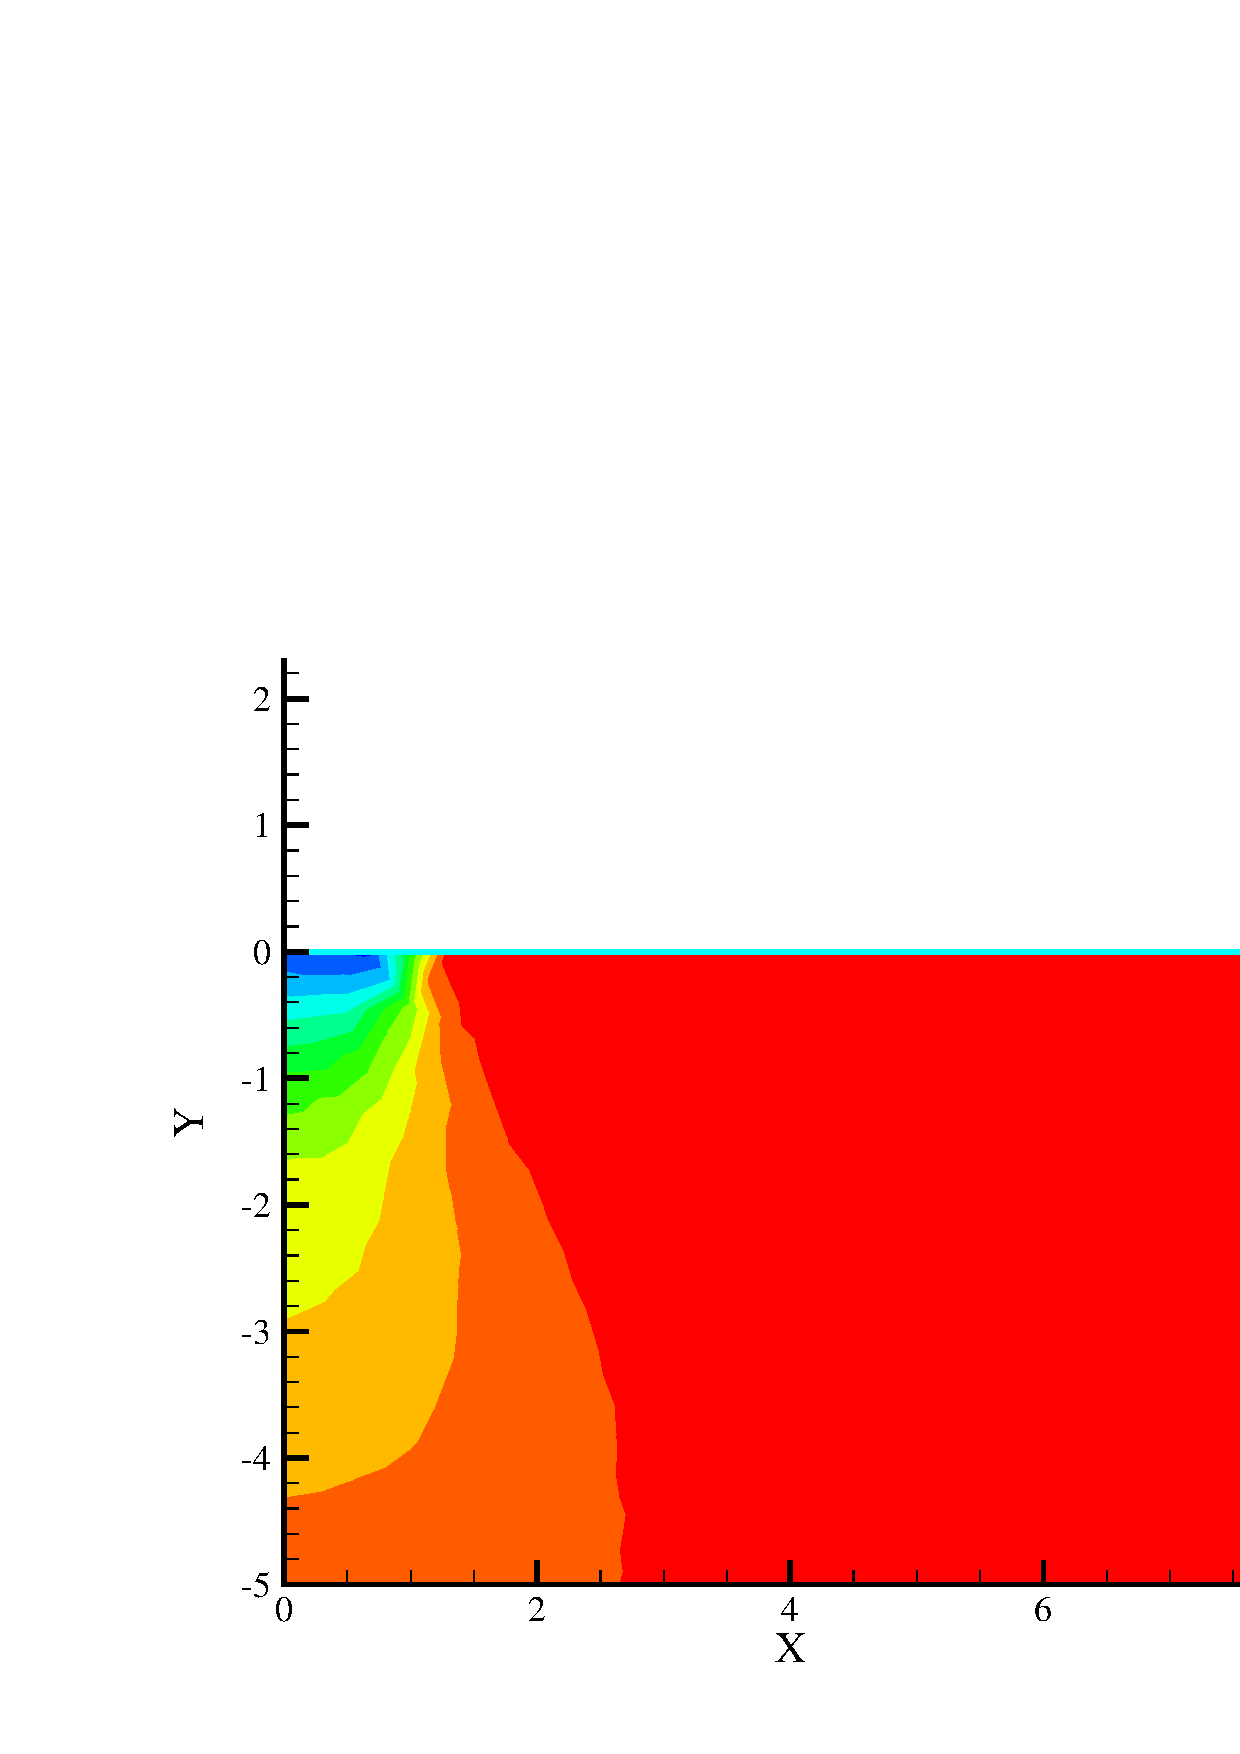
\includegraphics[width=0.5\textwidth]{chapter_14/figures/fig_14_1_11}
\end{center}
\caption{Vertical stress.}
\label{fig_dynHM4}
\end{figure}












